\documentclass[11pt, a4paper]{article}
\usepackage{graphicx} % Required for inserting images
% \usepackage{float} % For option 'H' of figure environment
% \usepackage[section]{placeins} % Forces images (probably floats in general)
% to stay inside the section are in the code
\usepackage{caption} % for captions
\usepackage{bbm} % Math font; use \mathbbm{}
\usepackage[acronym]{glossaries} % for acronyms
\usepackage{physics} % Physics symbols

\usepackage{showlabels} % To show equations labels on the PDF. Comment at the end

% Defining acronyms
\newacronym{aeq}{AE}{Advection Equation}
\newacronym{laxf}{LAX-F}{Lax-Friedrichs}
\newacronym{laxw}{LAX-W}{Lax-Wendroff}
\newacronym{beq}{BE}{Burgers' Equation}
\newacronym{fc}{FC}{Flux Conservative}
\newacronym{nfc}{NFC}{Non Flux Conservative}

% Defining variables
\newcommand\figltwocap{\(L_2\) norm; \(+\) are saved data points for comparison
with the initial \(C_f\) and \(J\) values}
\newcommand\figifcap{Initial and final conditions}

\title{Numerical Relativity Homework 1}
\author{Federico Leto di Priolo}
\date{May 2024}

\begin{document}

\maketitle

\section{\acrfull{aeq}}

The \acrshort{aeq} is the simplest study case of the hyperbolic partial
differential equation representing a conservation law. In 1D:\(\frac{\partial
    u}{\partial t} + \frac{\partial f(u)}{\partial u} \frac{\partial u}{\partial x}
= 0\); setting \(f(u) = au\) where \(a \in \mathbbm{R}\) leads to:

\begin{equation} \label{eq:adv_eq}
    \pdv{u}{u} + a \pdv{u}{x} = 0
\end{equation}

\noindent
The solution of the \acrshort{aeq} is a translation of the initial solution
\(u(t = 0,\ x)\) with constant velocity \(a\); if \(a > 0\):

\begin{equation} \label{eq:adv_sol}
    u(t,\ x) = u(t = 0,\ x - at)
\end{equation}

Since the \acrshort{aeq} doesn't affect the shape and amplitude of the solution
as time advance, we expect its norm to be conserved. Therefore we will use the
\(L_2\) norm to test the stability of the numerical methods used to evolve the
solution. On a discrete space-time grid it can be written as:

\begin{equation} \label{eq:l2_norm}
    \norm{u^n_j}_2 = \qty(\frac{1}{J} \sum_{i = 1}^J \abs{u^n_i}^2)^\frac{1}{2}
\end{equation}

\noindent
where \(u^n_j = u(t^n,\ x_j)\), \(J\) is the total number of points in the space
domain and \(n\) is the time index at which we are evaluating the solution.

For this exercise the initial condition is a \textbf{Gaussian profile} set to
\(u(t = 0,\ x) = \exp(-(x - x_0)^2)\) with \(x_0 = 5\), to be solved on a grid
with extent \(x \in [0, 10]\) up to \(t = 20\). Initially the Courant factor is
set to \(C_f = 0.5\) and the number of points to \(J = 101\), corresponding to
a resolution of \(10 / (J - 1) = 0.1\). Those have been varied to check the
behavior of the numerical methods. The speed \(a\) is set to \(1\).

In every \(L_2\) norm plot the norm its self has been normalized to its initial
value to facilitate the comparison between results obtained with different
values of \(J\) and \(C_f\).

\subsection{FTCS}

\begin{equation} \label{eq:ftcs}
    u^{n+1}_j = u^n_j - \frac{a \Delta t}{2 \Delta x} (u^n_{j+1} - u^n_{j-1})
\end{equation}

The FTCS method is unconditionally unstable and we expect the solution to
explode after a sufficient number of time steps. An example of what the
solution at the final time looks compared to the initial profile can be seen in
Figure \ref{fig:ftcs_if_1}. Changing the Courant factor and the number of grid
points influences the rapidity of the \textit{explosion} as can be see in
Figure \ref{fig:ftcs_l2_tot}.

\begin{center}
    \centering
    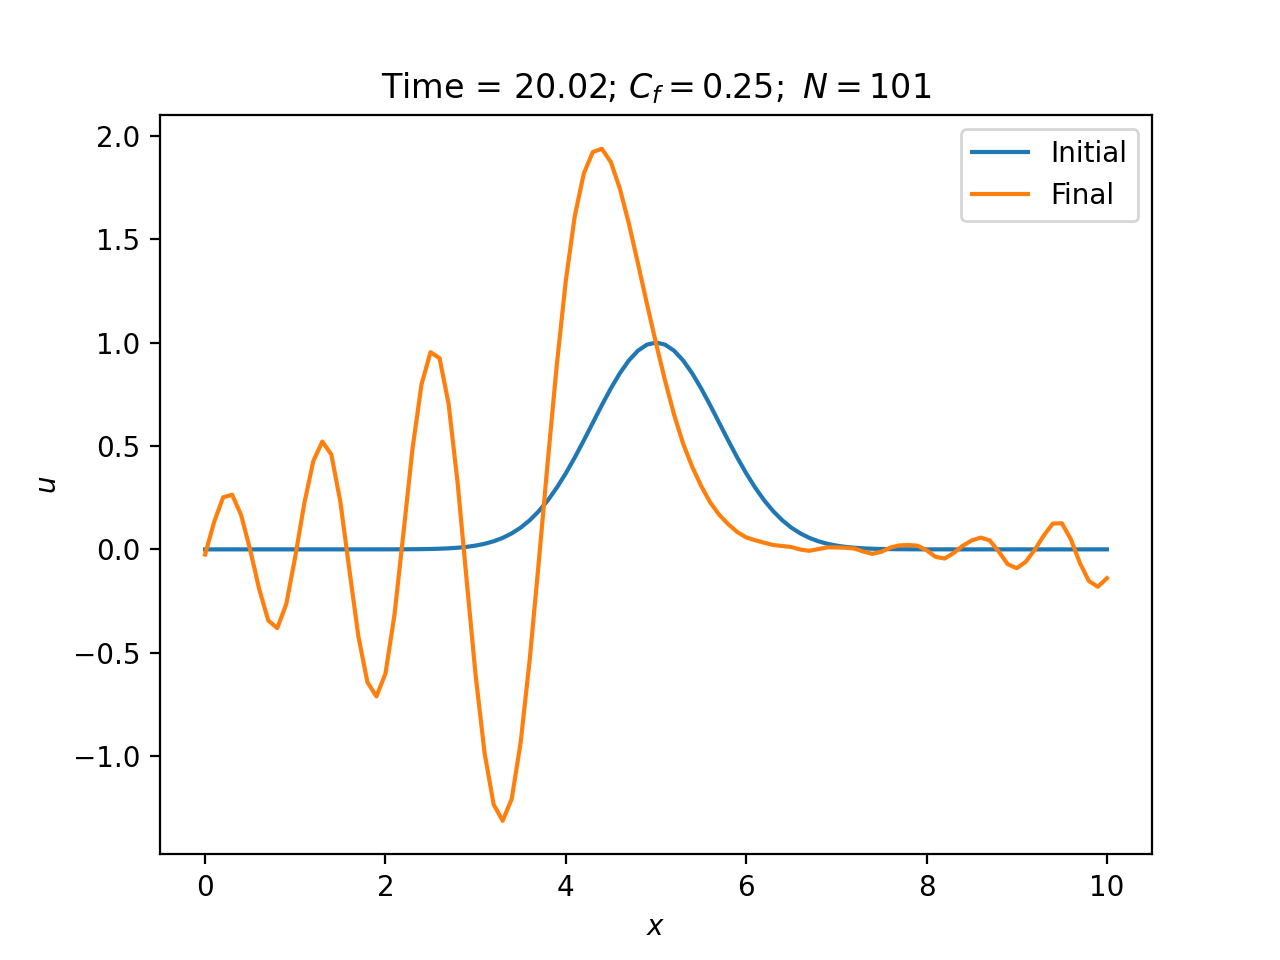
\includegraphics[width=0.9\linewidth]{images/IF_Cf-0.25_N-101.png}
    \captionof{figure}{FTCS; \figifcap.}
    \label{fig:ftcs_if_1}
\end{center}

\begin{center}
    \centering
    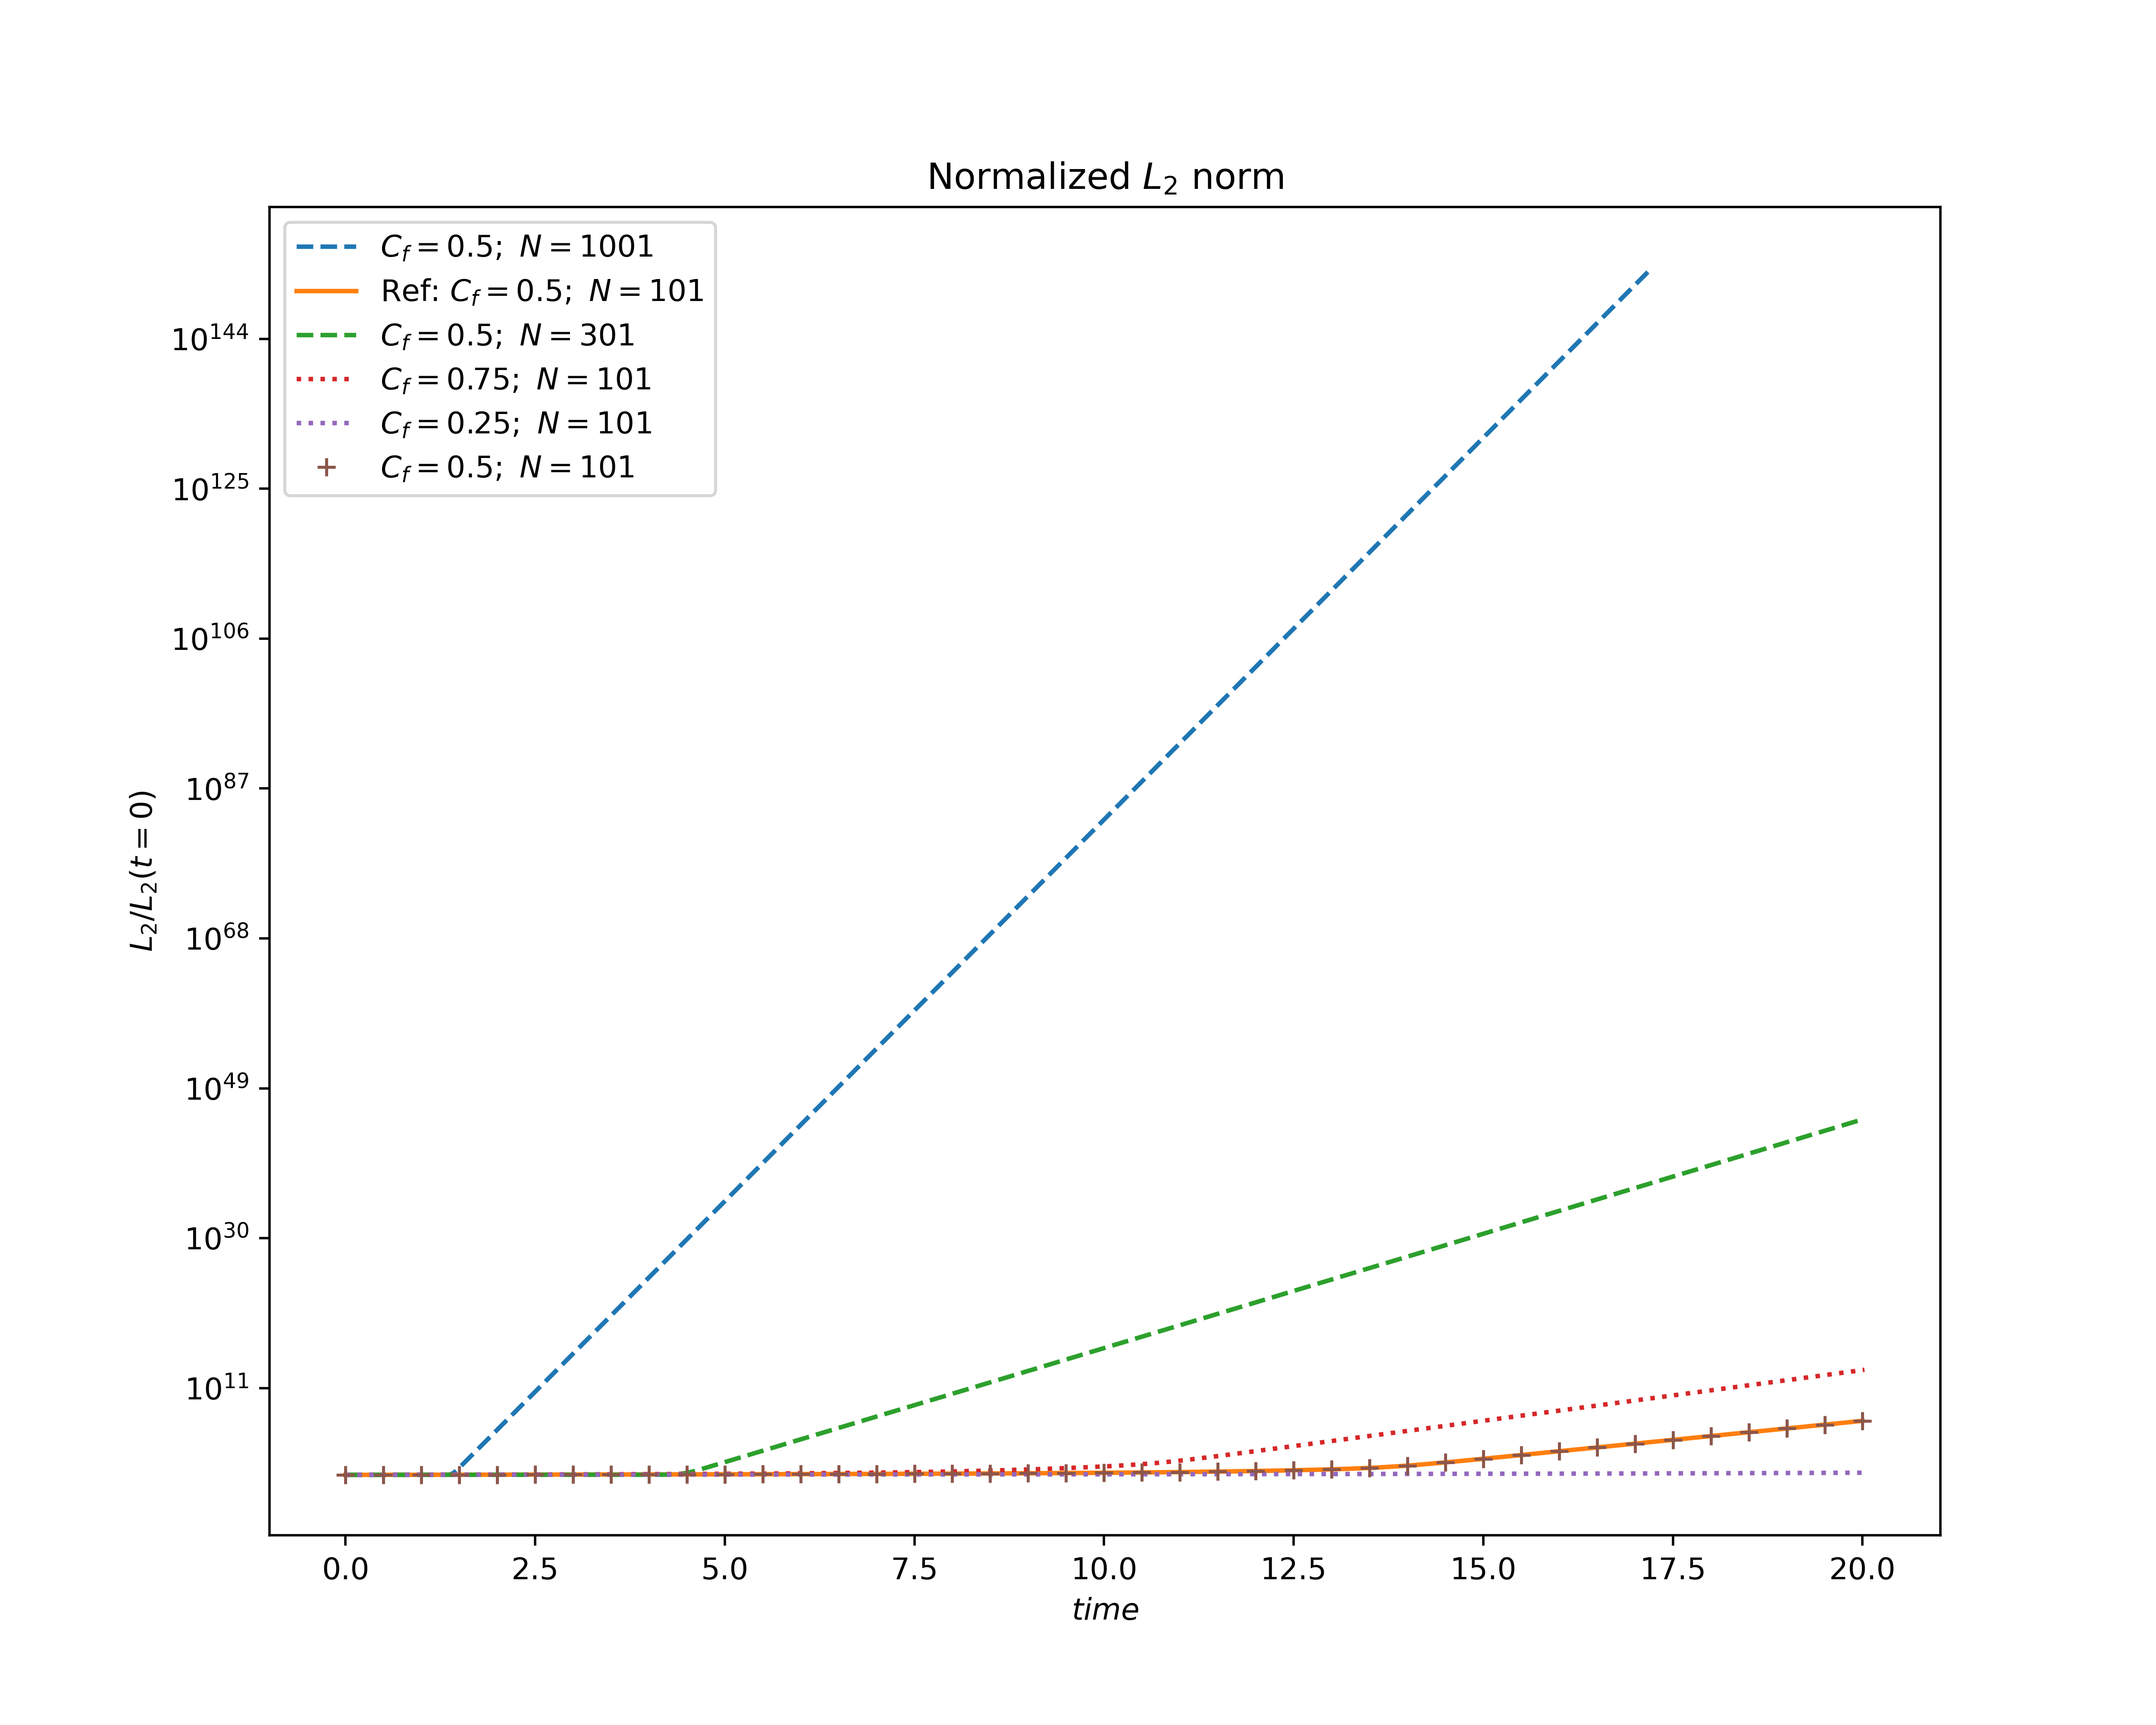
\includegraphics[width=0.9\linewidth]{images/L2_GAUS_FTCS.png}
    \captionof{figure}{FTCS; \figltwocap.}
    \label{fig:ftcs_l2_tot}
\end{center}

\subsection{\acrfull{laxf}}

\begin{equation} \label{eq:lax-f}
    u^{n+1}_j = \frac{1}{2}(u^n_{j-1} + u^n_{j+1}) - \frac{a \Delta t}{2 \Delta x} (u^n_{j+1} - u^n_{j-1})
\end{equation}

The \acrshort{laxf} method is conditionally stable; the stability condition is
given by \(\Delta t = C_f \frac{\Delta x}{\abs{a}}\) with \(C_f \leq 1\). The
derivation of this method is achieved with the introduction of a
\textit{dissipative} term in the \acrshort{aeq}; this means that the amplitude
of the solution decreases in time depending on the Courant factor and the
number of grid points.

As can be seen from Figure \ref{fig:laxf_if_tot}, increasing the resolution of
the grid or the Courant factor helps in preserving the initial amplitude of the
solution. These features are also present in the evolution of the \(L_2\) norm
(Figure \ref{fig:laxf_l2_tot}). Further comments are in section
\ref{sec:step_laxf}.

\begin{center}
    \centering
    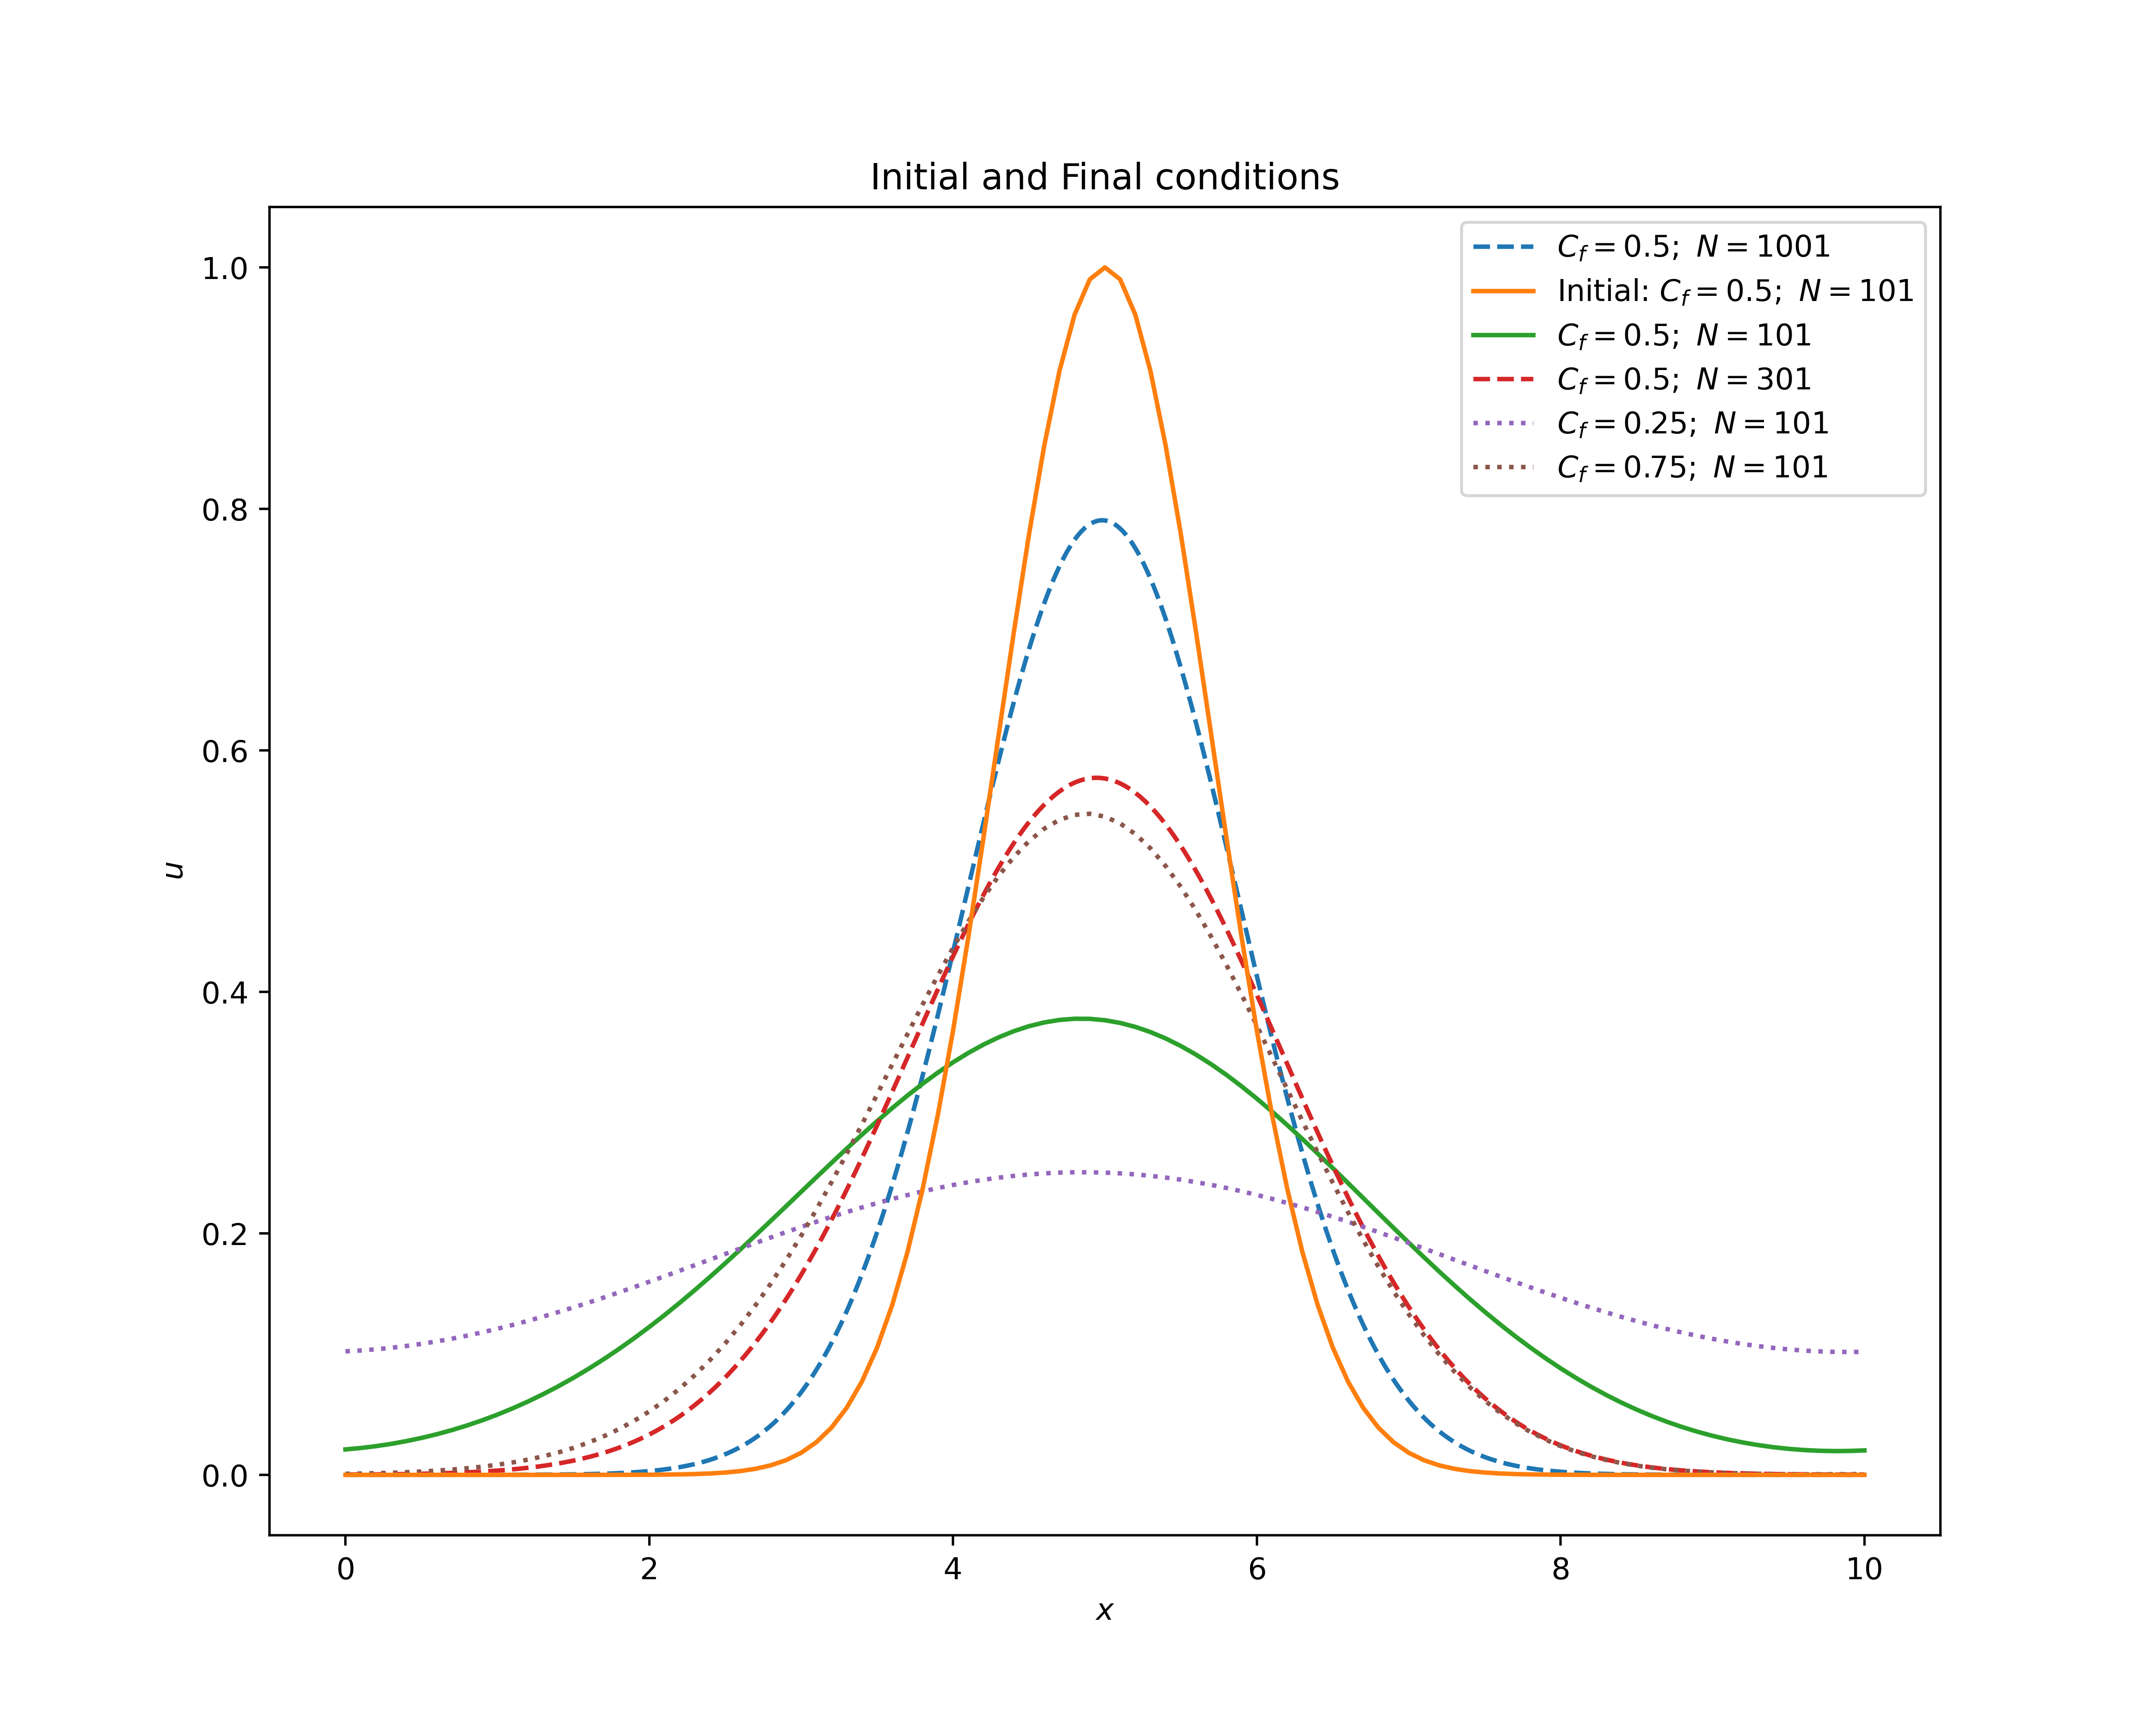
\includegraphics[width=0.9\linewidth]{images/IF_GAUS_LAX-F.png}
    \captionof{figure}{\acrshort{laxf}; \figifcap.}
    \label{fig:laxf_if_tot}
\end{center}

\begin{center}
    \centering
    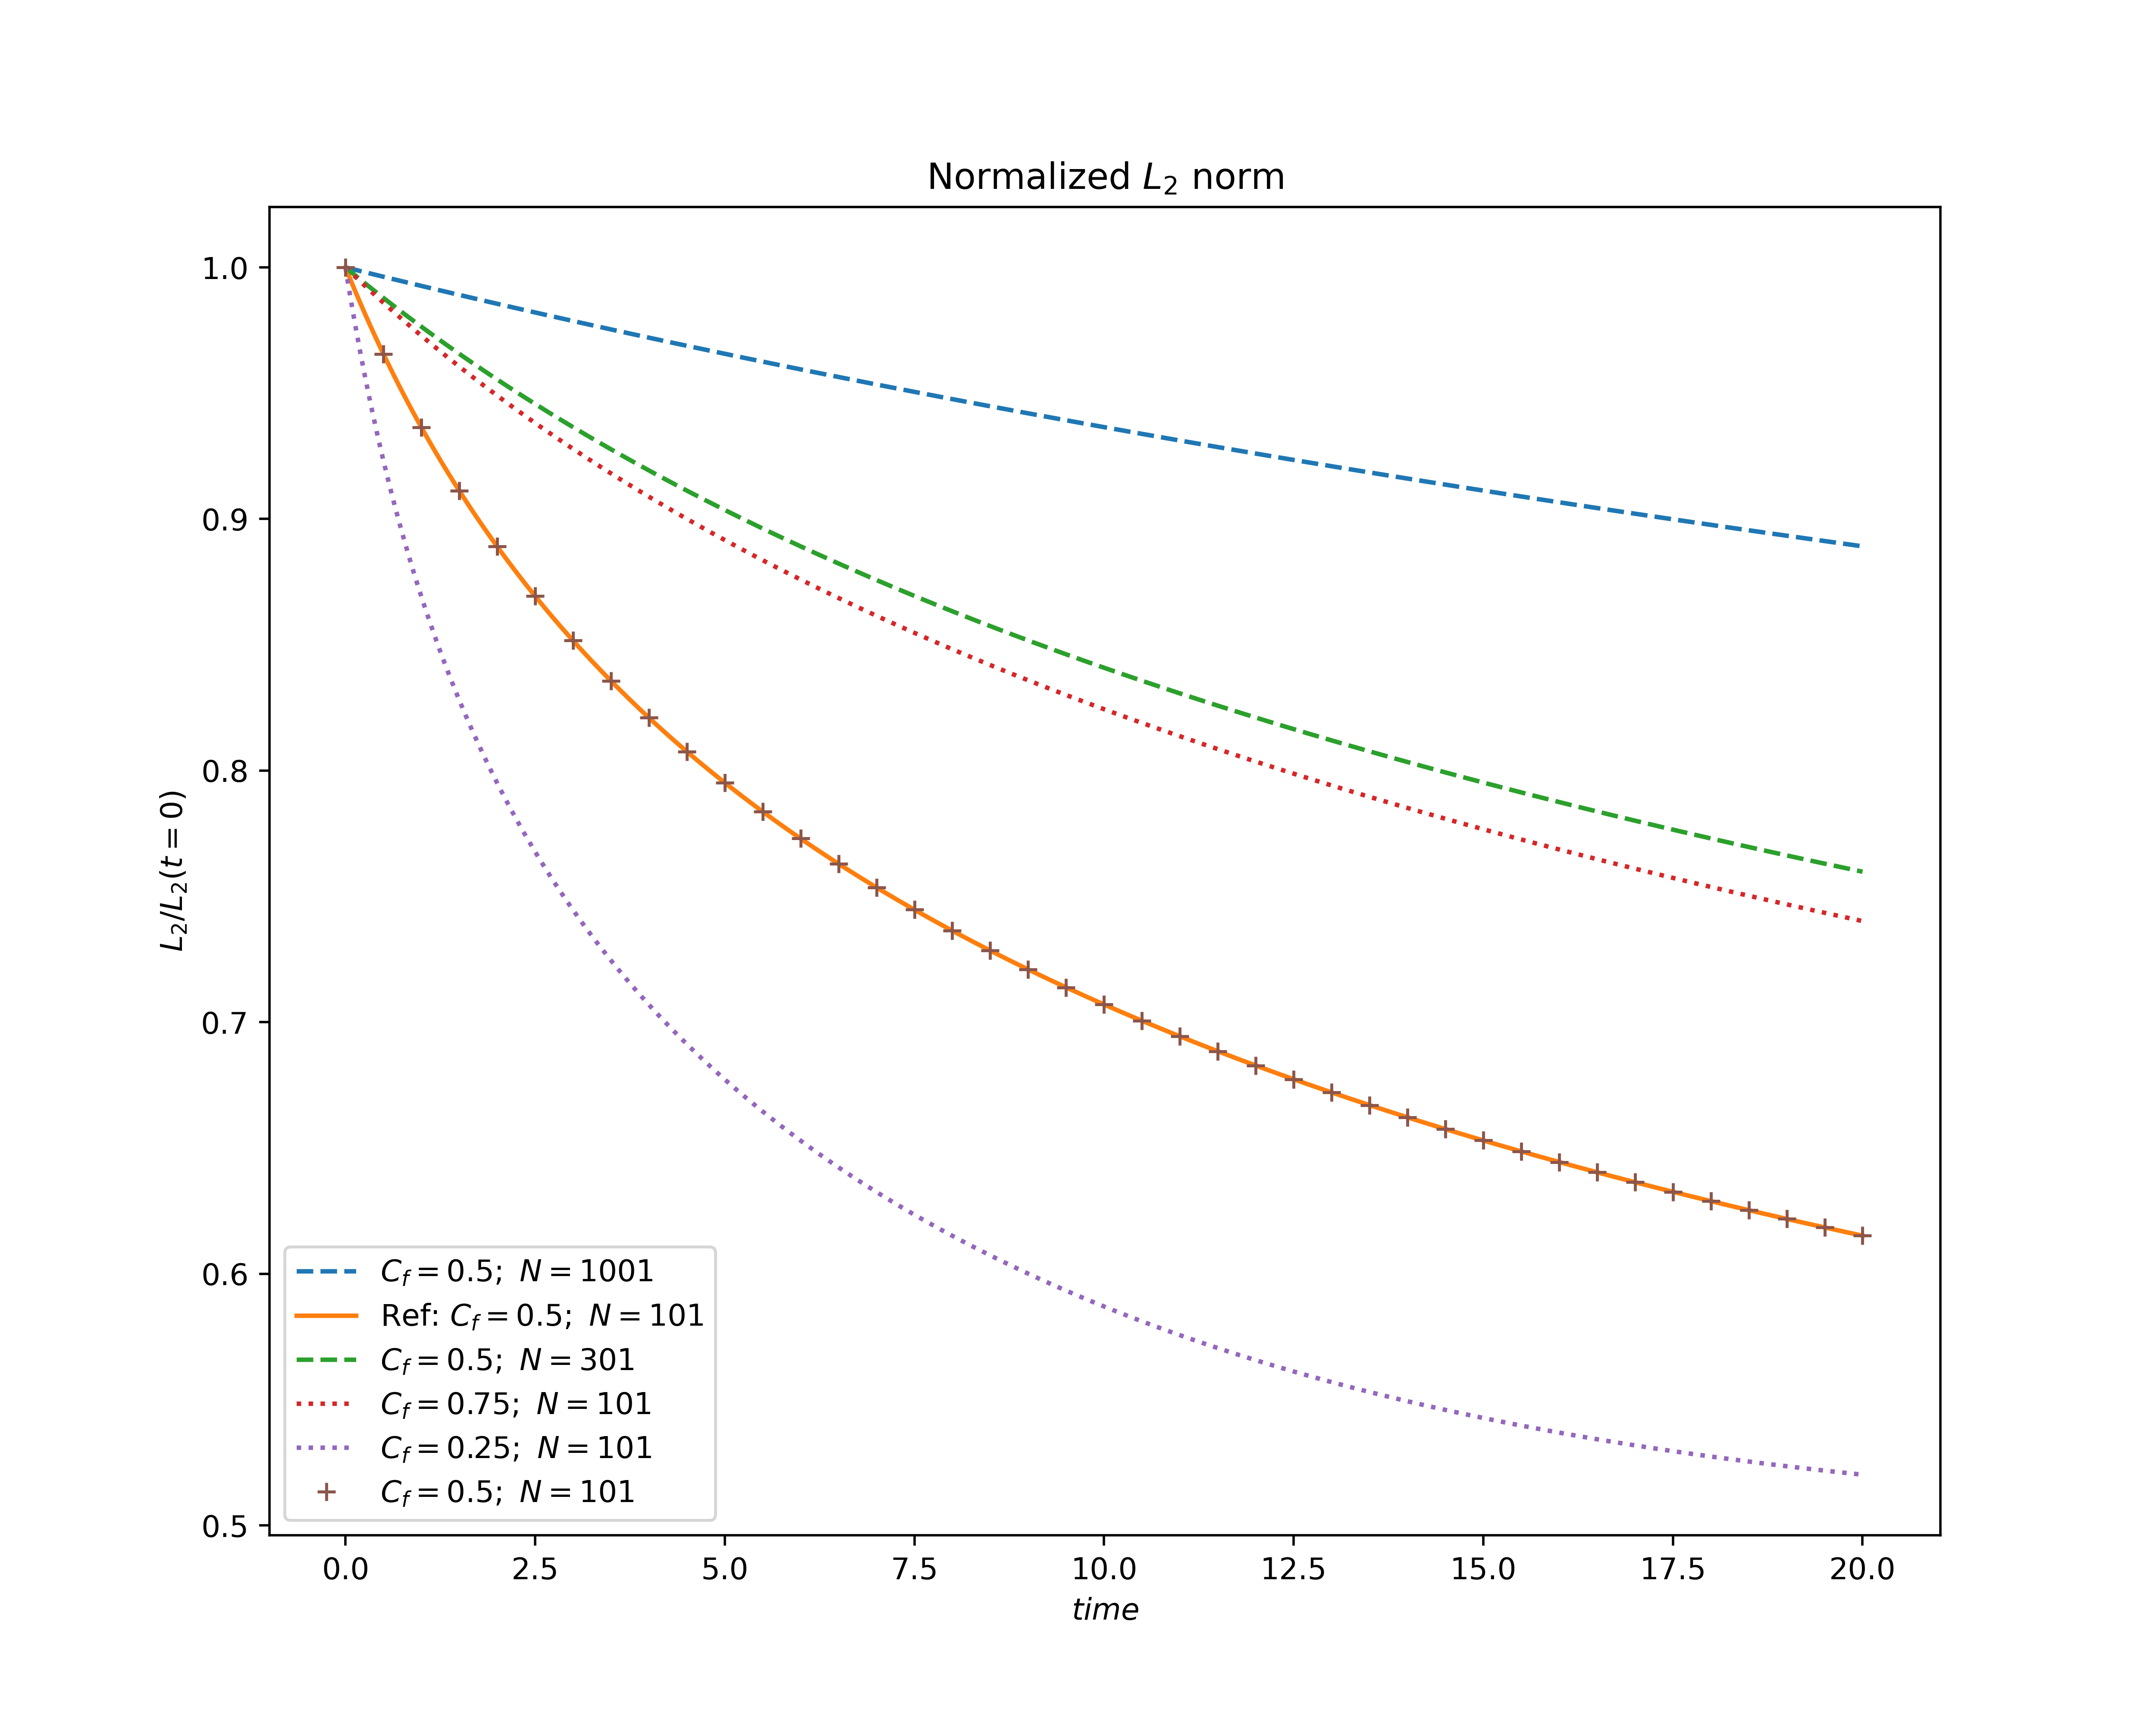
\includegraphics[width=0.9\linewidth]{images/L2_GAUS_LAX-F.png}
    \captionof{figure}{\acrshort{laxf}; \figltwocap.}
    \label{fig:laxf_l2_tot}
\end{center}

\subsection{Leapfrog}

\begin{equation} \label{eq:leapfrog}
    u^{n+1}_j = u^{n-1}_j - \frac{a \Delta t}{\Delta x} (u^n_{j+1} - u^n_{j-1})
\end{equation}

Like the \acrshort{laxf}, the Leapfrog method is stable for \(C_f \leq 1\). The
main difference of this compared with the others is that it involves 3 time
levels at each step: the next step is computed as a function of the current
step and of the previous one. For the first time step (which relies on the
value of \(u\) one step before the initial time \(t = 0\)) the solution has
been computed using the \acrshort{laxf} method. The \(L_2\) shows oscillations
with an amplitude that depends on the resolution and the Courant factor (Figure
\ref{fig:leapfrog_l2_tot}).

\begin{center}
    \centering
    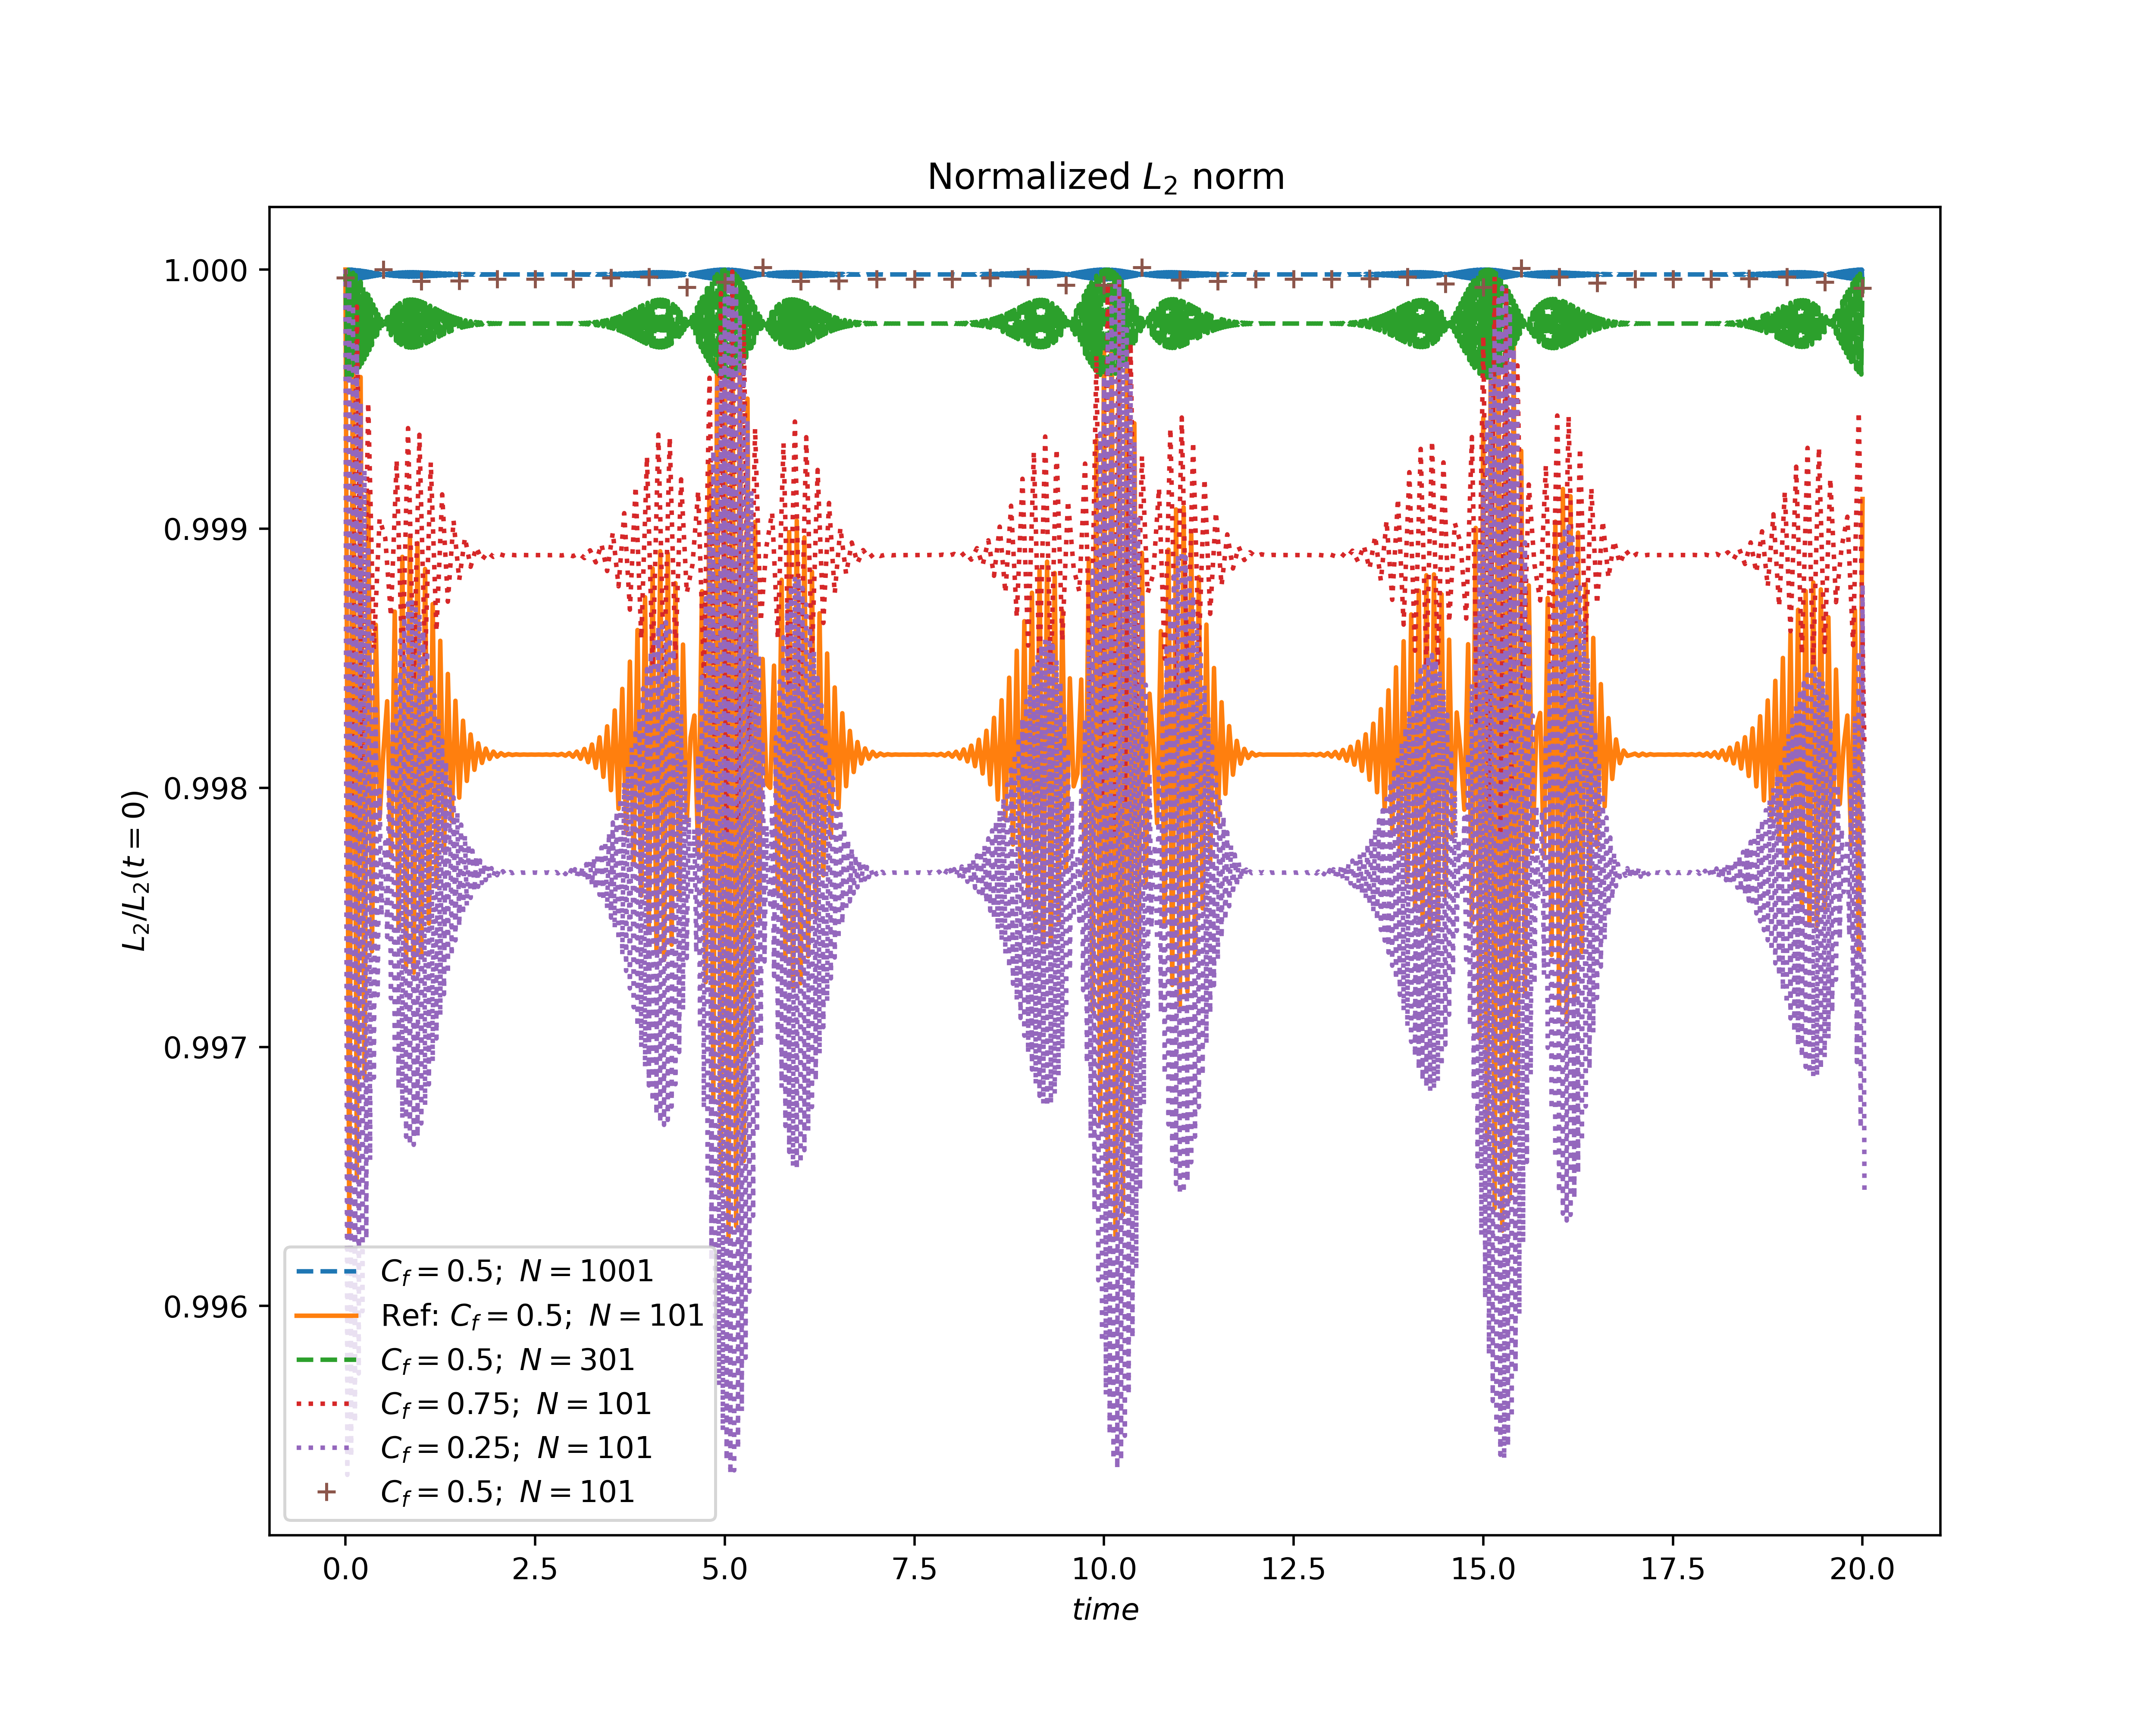
\includegraphics[width=0.9\linewidth]{images/L2_GAUS_LEAPFROG.png}
    \captionof{figure}{Leapfrog; \(L_2\) norm.}
    \label{fig:leapfrog_l2_tot}
\end{center}

\subsection{\acrfull{laxw}}

\begin{equation} \label{eq:lax-w}
    u^{n+1}_j = u^n_j - \frac{a \Delta t}{2 \Delta x} (u^n_{j+1} - u^n_{j-1}) + \frac{1}{2}\qty(\frac{a \Delta t}{\Delta x})^2 (u^n_{j+1} - 2u^n_j + u^n_{j-1})
\end{equation}

The \acrshort{laxw} scheme is a combination of the \acrshort{laxf} and the
Leapfrog. Its main new feature is the introduction of a \textit{dispersive}
term in the \acrshort{aeq}. The dissipative term from the \acrshort{laxf} is
still there, but is subdominant. The final solutions computed with this method
with different values of the resolution and \(C_f\) can be seen in Figure
\ref{fig:laxw_if_tot}. As expected the strong dissipation observed for the
\acrshort{laxf} method doesn't occur; instead, we can see the effect of the
dispersive term on the left side of the Gaussian profile.

In this case the dependence of the \(L_2\) norm from the Courant factor is
different from the \acrshort{laxf} case because it appears in a more
complicated way in the Von Neumann stability analysis. Figure
\ref{fig:laxw_l2_tot} shows the evolution of the \(L_2\) norm for the cases of
Figure \ref{fig:laxw_if_tot}. It appears that the main behavior of the norm is
driven by the the used resolution rather than the choice of the Courant factor.
Further comments are in section \ref{sec:step_laxw}.

\begin{center}
    \centering
    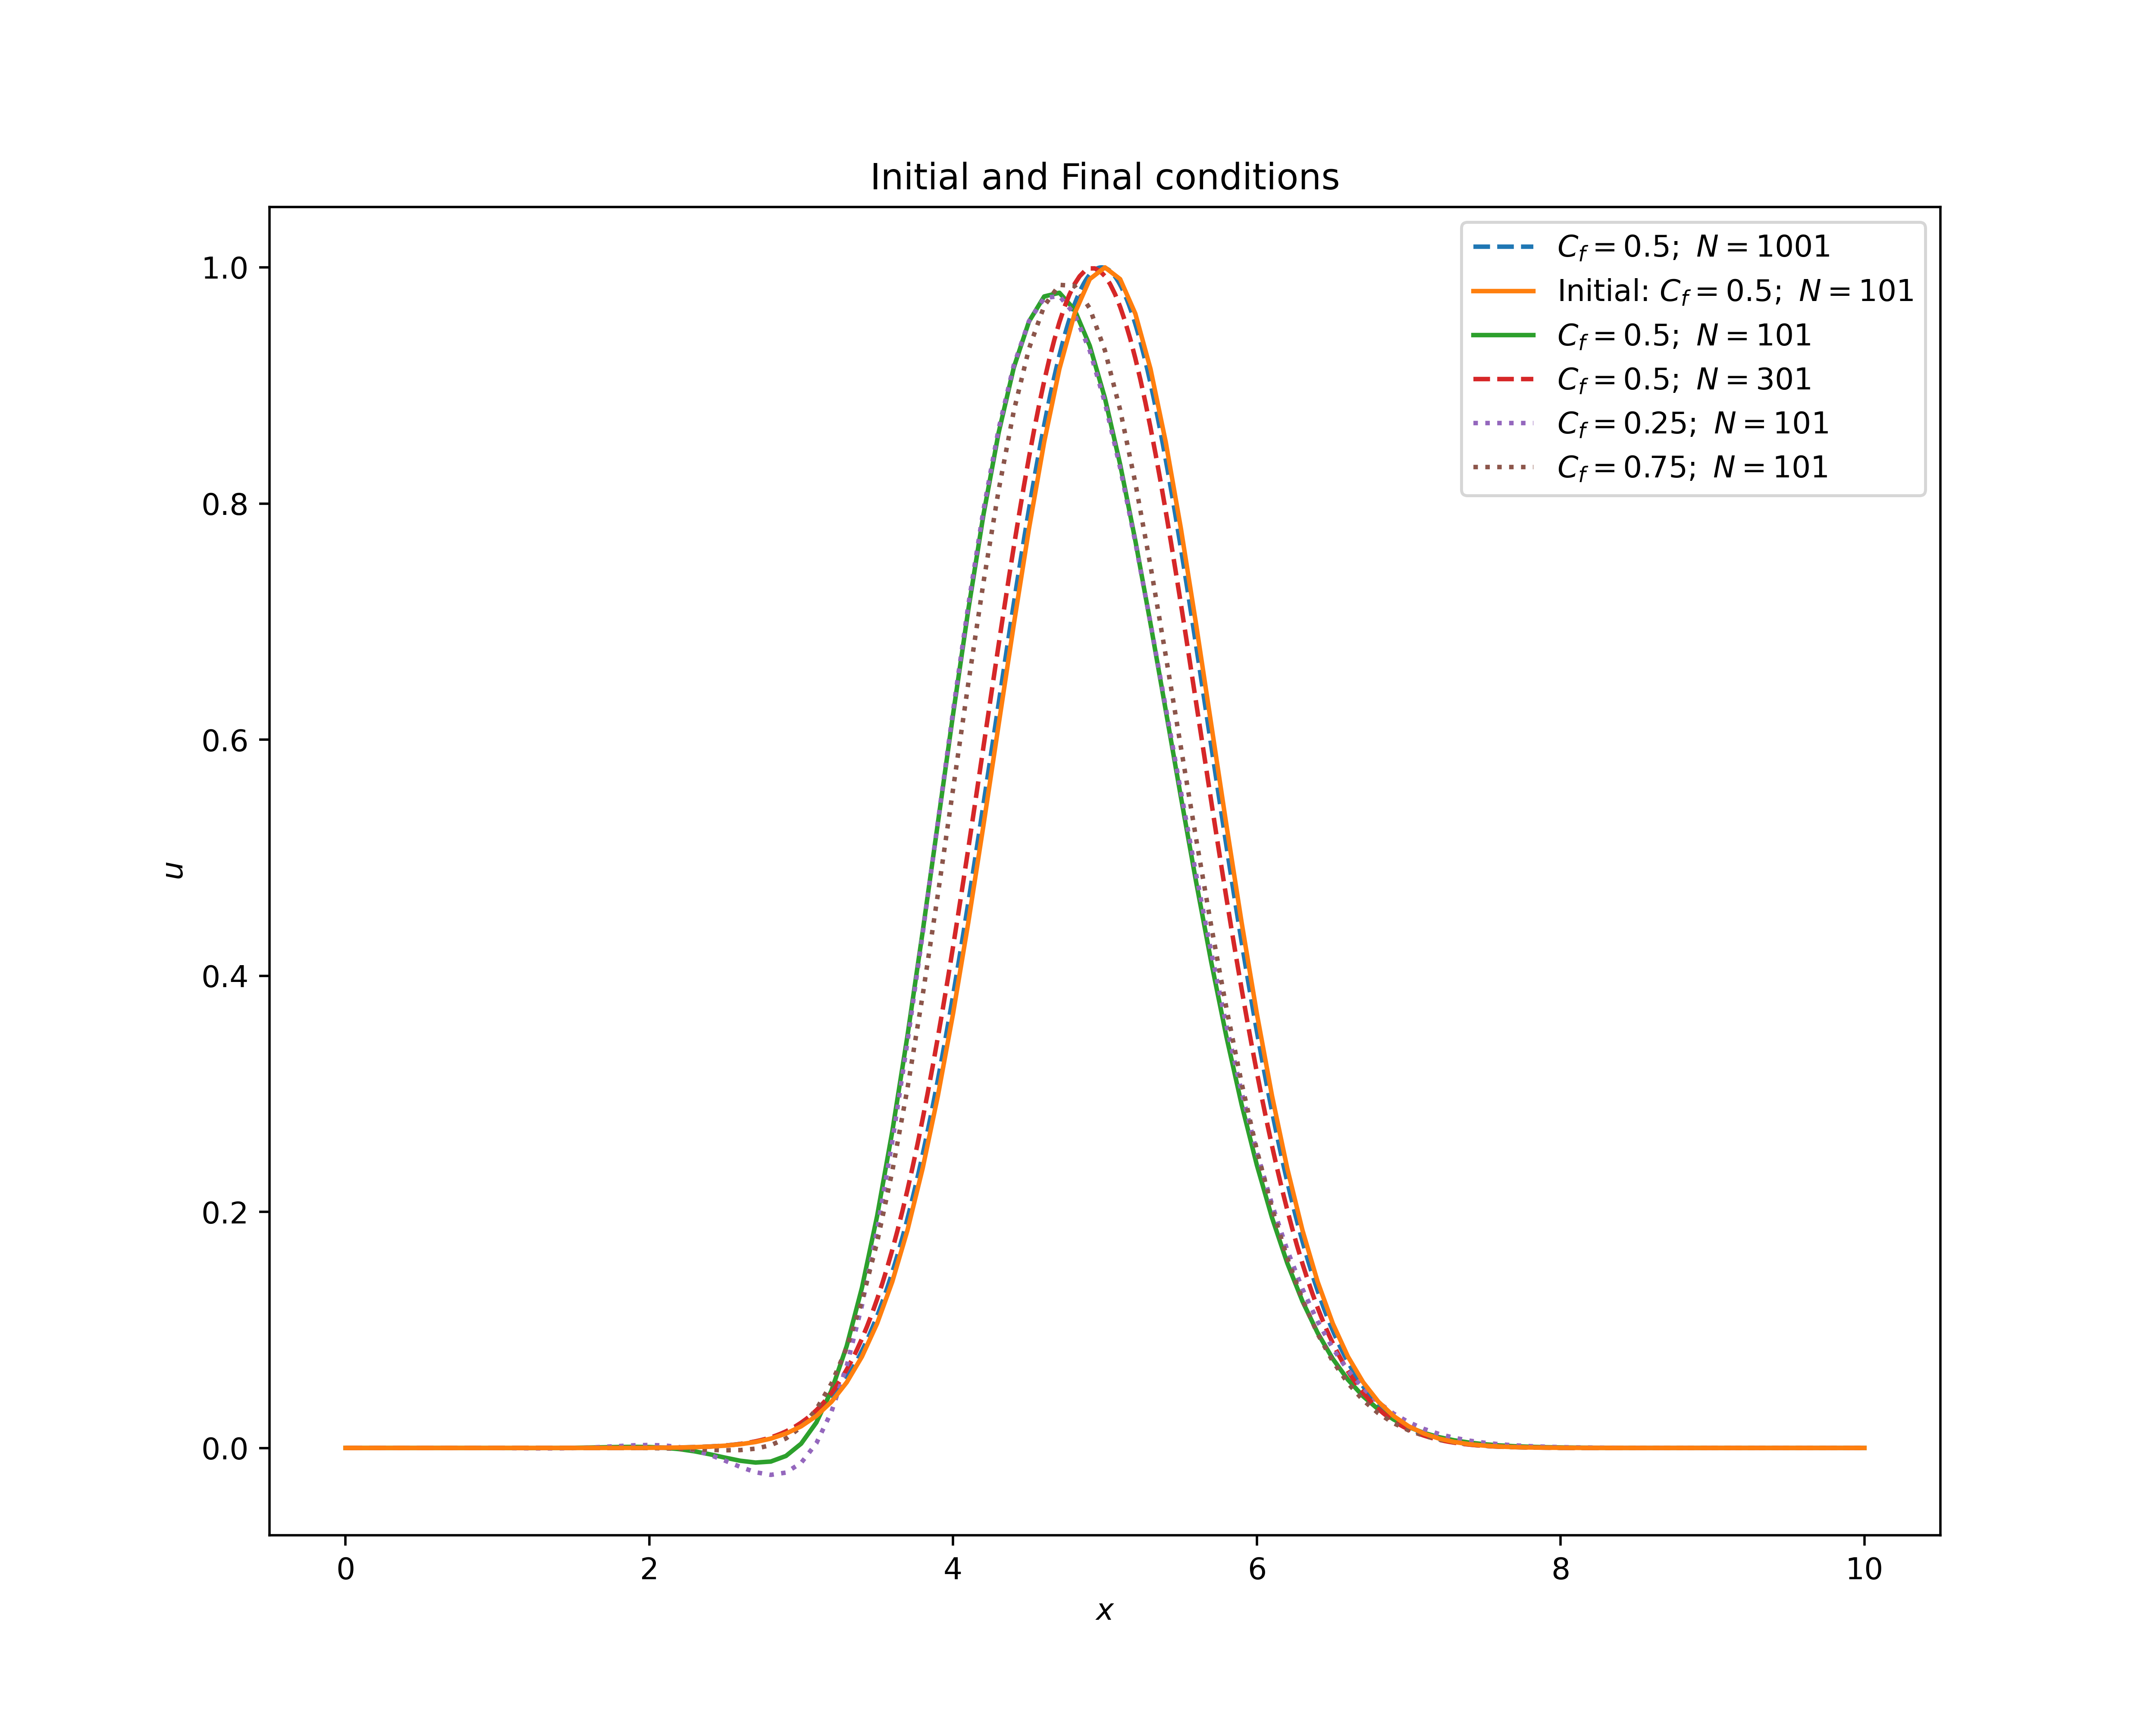
\includegraphics[width=0.9\linewidth]{images/IF_GAUS_LAX-W.png}
    \captionof{figure}{\acrshort{laxw}; \figifcap.}
    \label{fig:laxw_if_tot}
\end{center}

\begin{center}
    \centering
    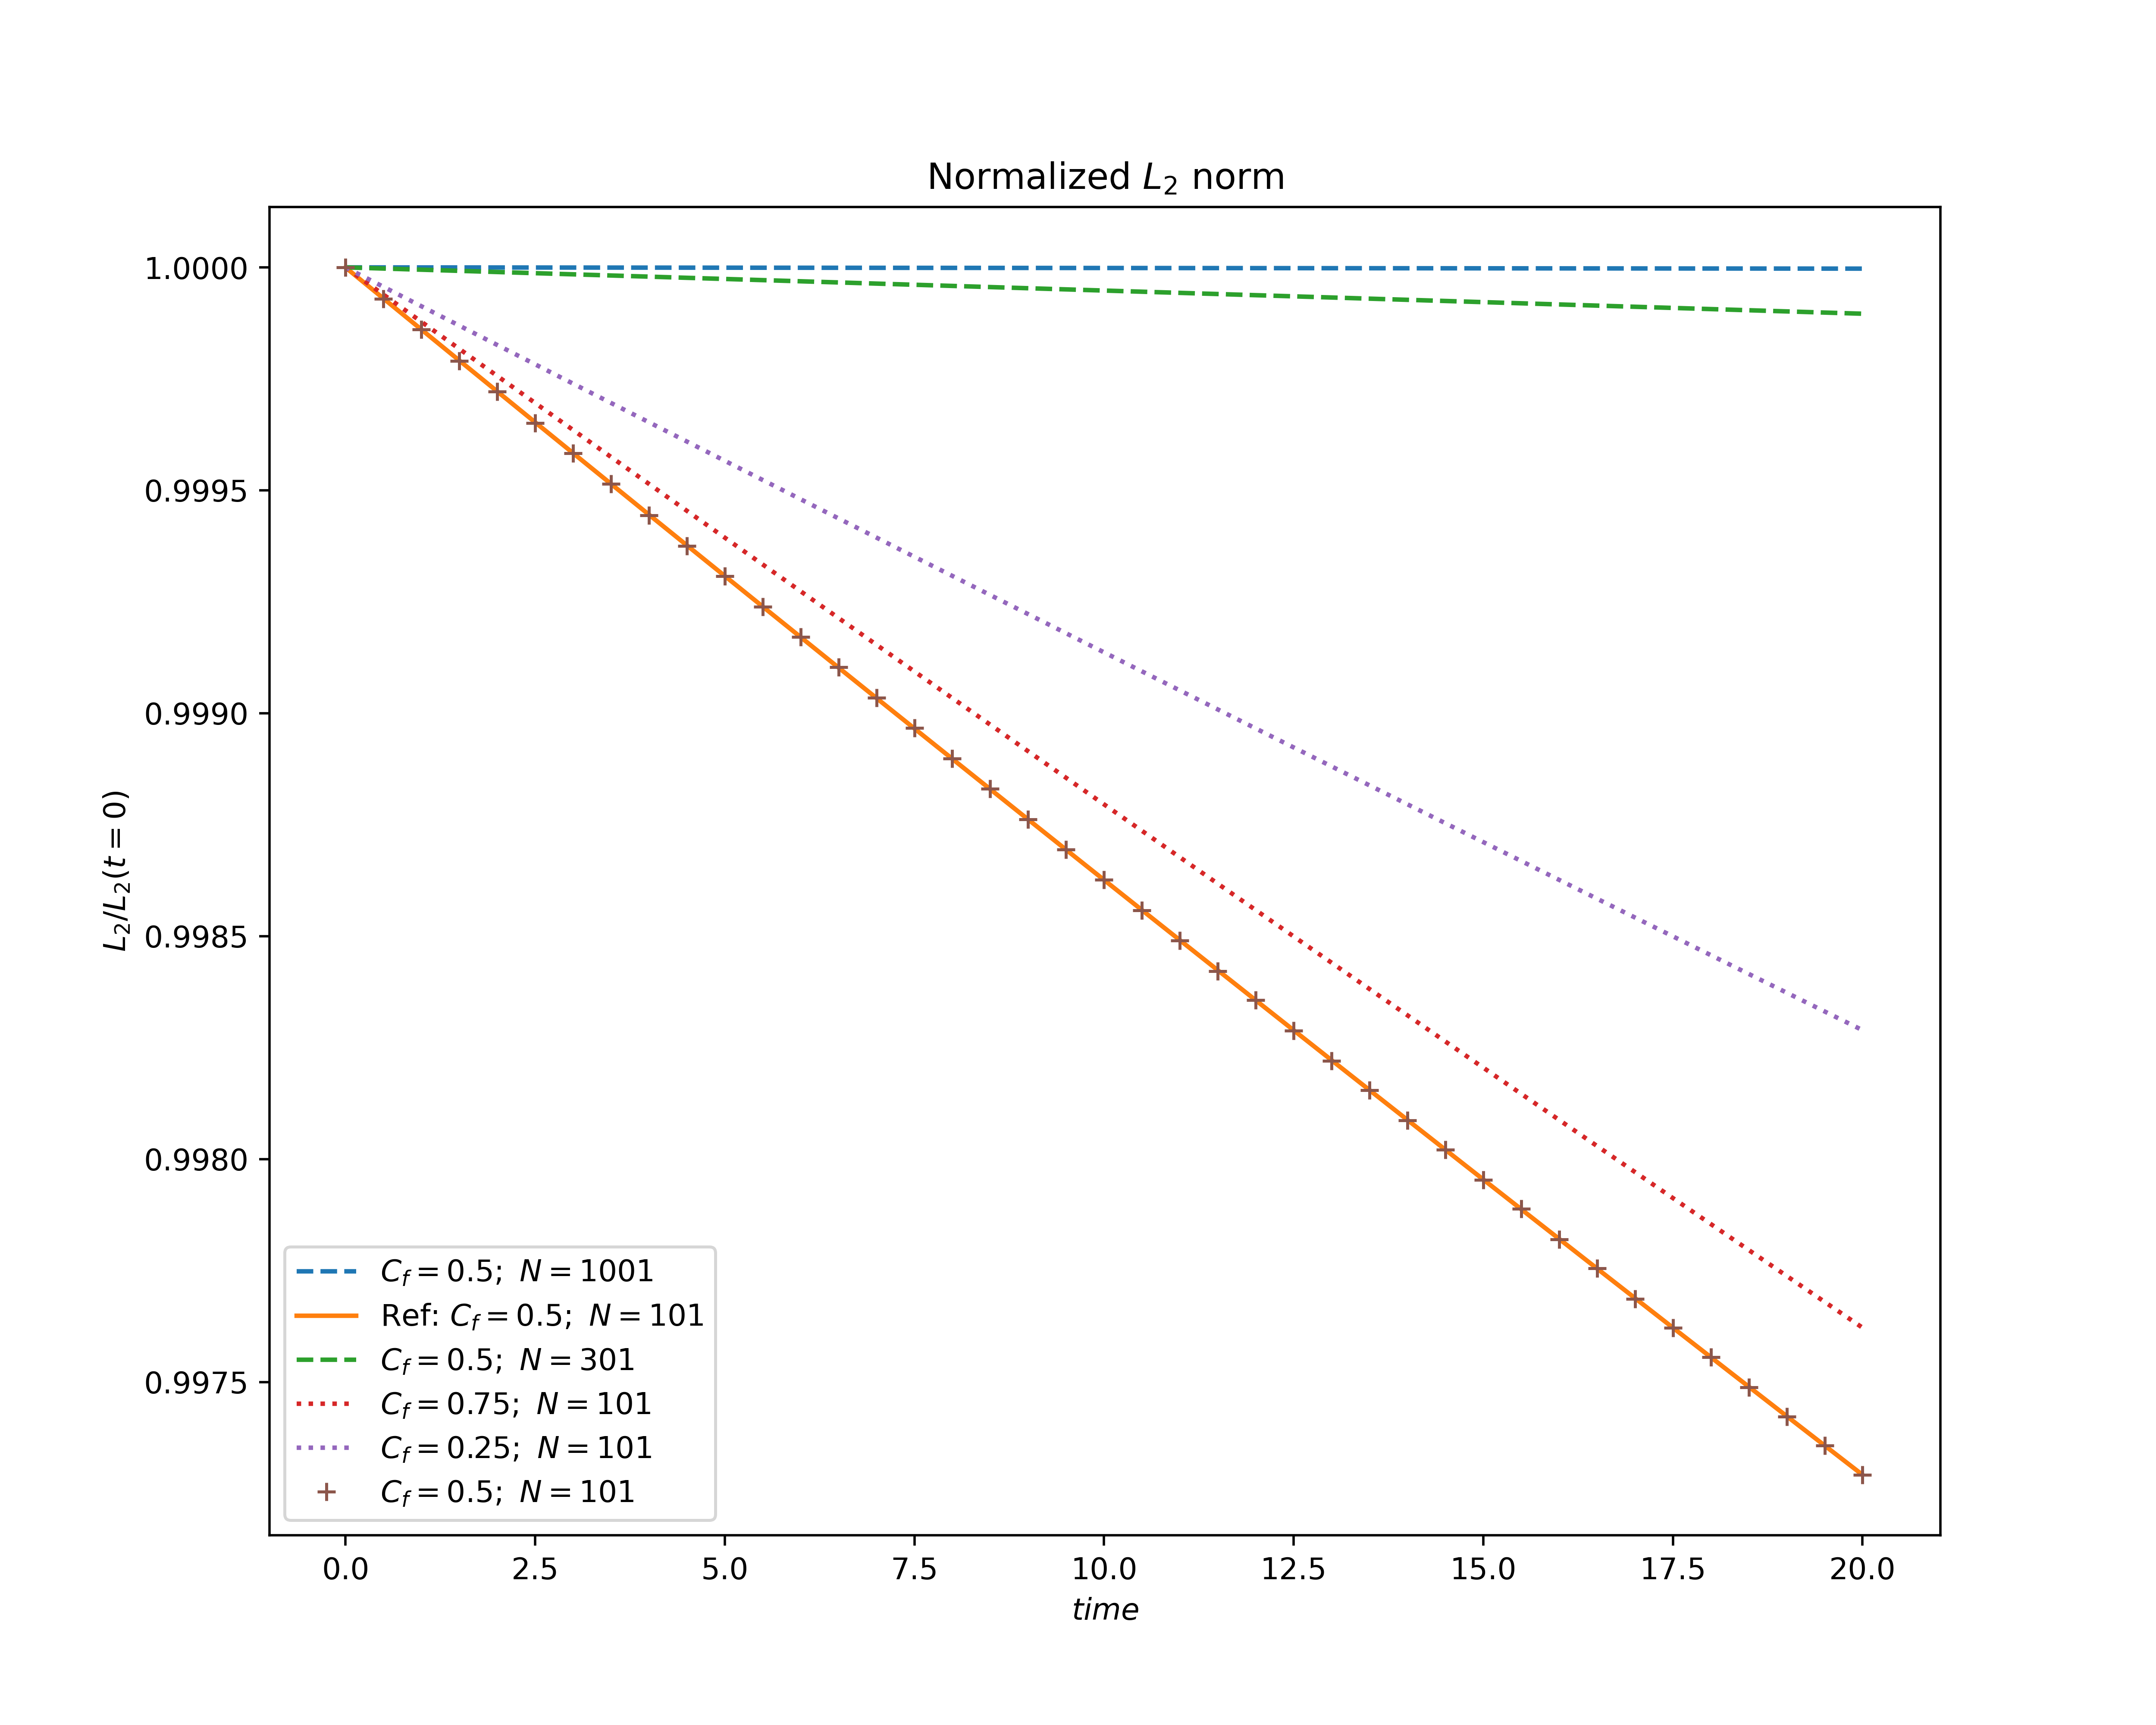
\includegraphics[width=0.9\linewidth]{images/L2_GAUS_LAX-W.png}
    \captionof{figure}{\acrshort{laxw}; \figltwocap.}
    \label{fig:laxw_l2_tot}
\end{center}

\section{Step Function}

The aim now is to solve the \acrshort{aeq} replacing the Gaussian profile with
a \textbf{Step Function}: \(u(t = 0,\ x) = 1\) for \(x \in [4, 6]\) and \(0\)
elsewhere. The other parameters are left unchanged but for the number of points
and the Courant factor that will be varied as has been done before. We will use
the \acrlong{laxf} and the \acrlong{laxw} methods.

\subsection{\acrlong{laxf}} \label{sec:step_laxf}

In order to advance of one step the \acrshort{laxf} method takes the average of
the values on the left and on the right of each numerical cell. This is done by
the \(\frac{1}{2}(u^n_{j-1} + u^n_{j+1})\) term in Equation \ref{eq:lax-f}.
This means that when we apply it to the Step Function the edges of the
\textit{step} get weighted down and a new discontinuity is generated. At the
next iteration the new \textit{steps} are treated like the previous one,
generating new discontinuities, and so on.

Using a high resolution reduces the dissipation (like for the Gaussian profile)
and helps to keep the initial shape. A lower resolution instead spreads the
\textit{steps} profile on the wider domain of the individual cells. However,
the "spreading" is mainly controlled by the Courant factor: the higher the
Courant factor, the higher the time step, the lower is the number of iterations
and then the "spreading". Some example of the final shape of the solution
compared with the initial one are in Figure \ref{fig:step_laxf_if_tot}.

The evolution of the \(L_2\) norm is the same observed for the Gaussian profile
(Figure \ref{fig:laxf_l2_tot}).

\begin{center}
    \centering
    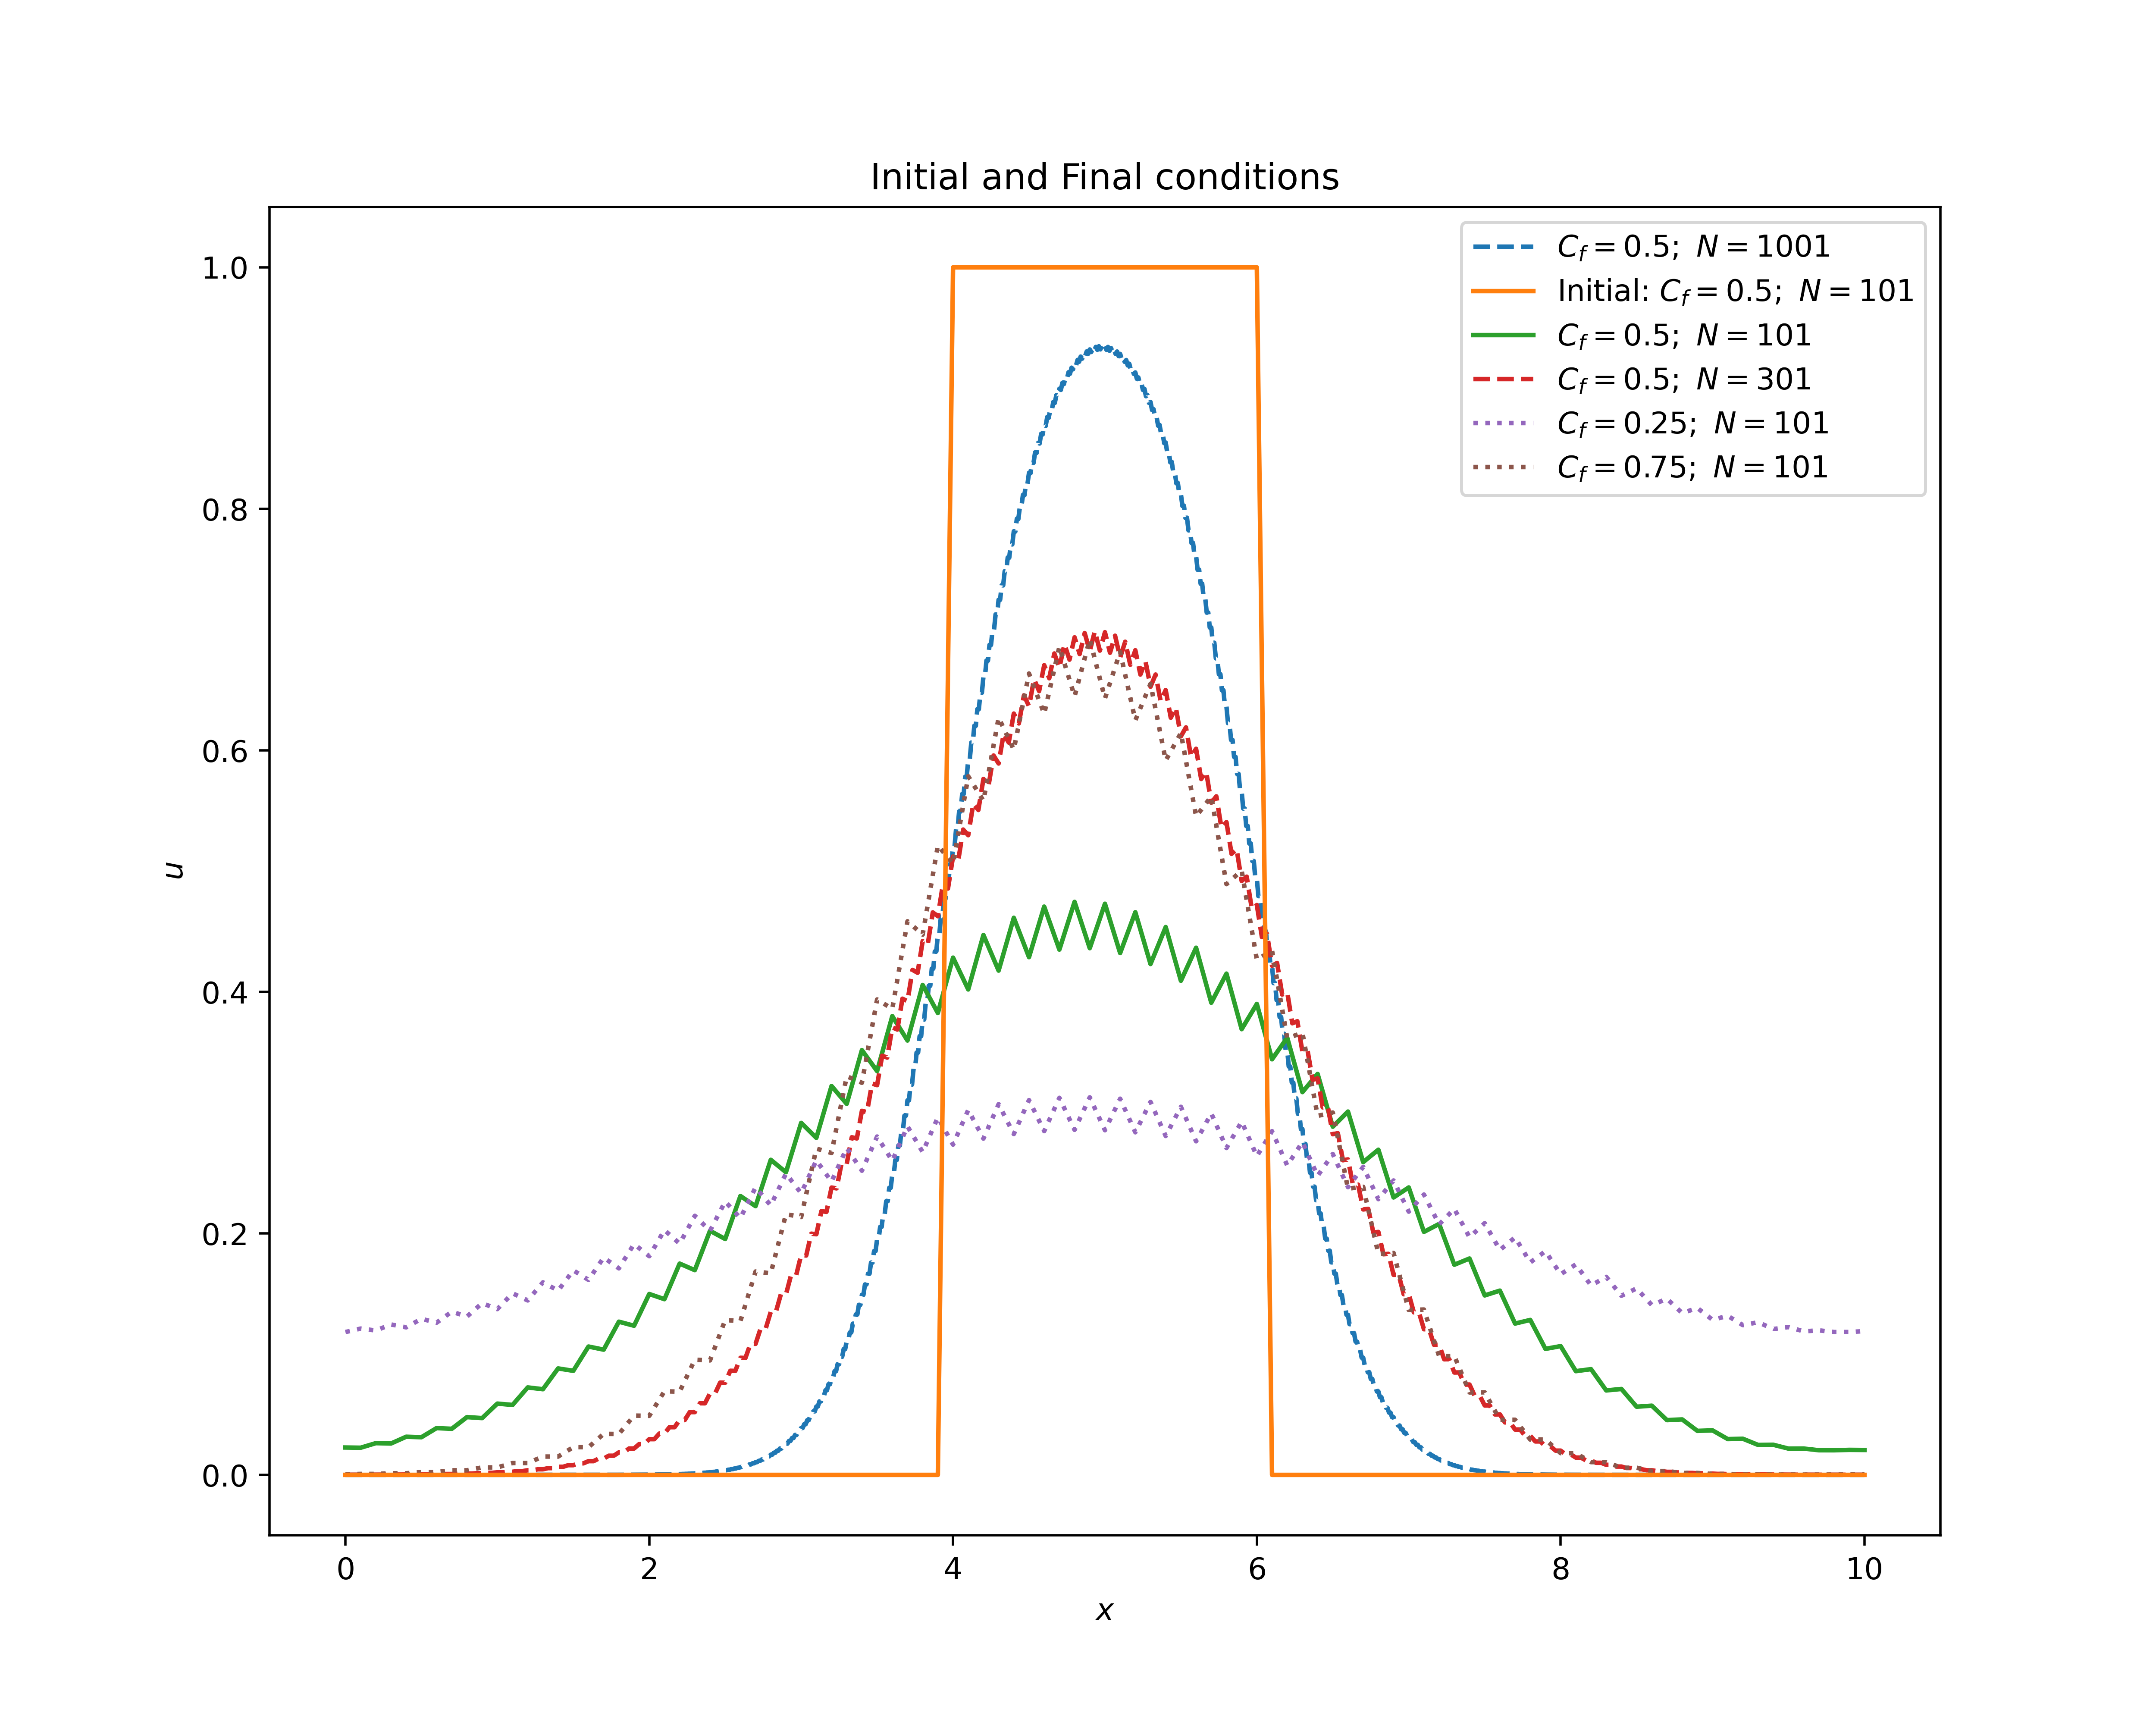
\includegraphics[width=0.9\linewidth]{images/IF_STEP_LAX-F.png}
    \captionof{figure}{Step Function; \acrshort{laxf}; \figifcap.}
    \label{fig:step_laxf_if_tot}
\end{center}

\subsection{\acrlong{laxw}} \label{sec:step_laxw}

If the \acrshort{laxf} method approximates the solution with piecewise
constant functions in every numerical cell, the \acrshort{laxw} also
introduces a slope to fit better the actual solution. The introduction of a
slope has the effect of generating oscillations in proximity of the
discontinuities (the \textit{steps}). That happens because the solution in each
cell is then represented with a line with a slope given by the incremental ratio
passing by the average value inside that cell. Moreover, we can recall
the \textbf{Godunov's Theorem}:

\begin{quote}
    Linear monotonic schemes are at most first order accurate.
\end{quote}

\noindent
Therefore, since the \acrshort{laxw} is linear and second order, we expect it
not to be monotonic and to develop new minima and maxima.

We expect the resolution to affect how much the oscillations are "spread": a
higher resolution (smaller cells) keeps the oscillations more confined near
the discontinuities. Figure \ref{fig:step_laxw_if_tot} shows the final solutions
for some choices of \(J\) and \(C_f\).

The evolution of the \(L_2\) norm (Figure \ref{fig:step_laxw_l2_tot}) is similar
to the one observed for the Gaussian profile, but for the shapes of the curves
that are not lines anymore. Like before the drop in amplitude of the norm is
mainly driven by the choice of the resolution.

\begin{center}
    \centering
    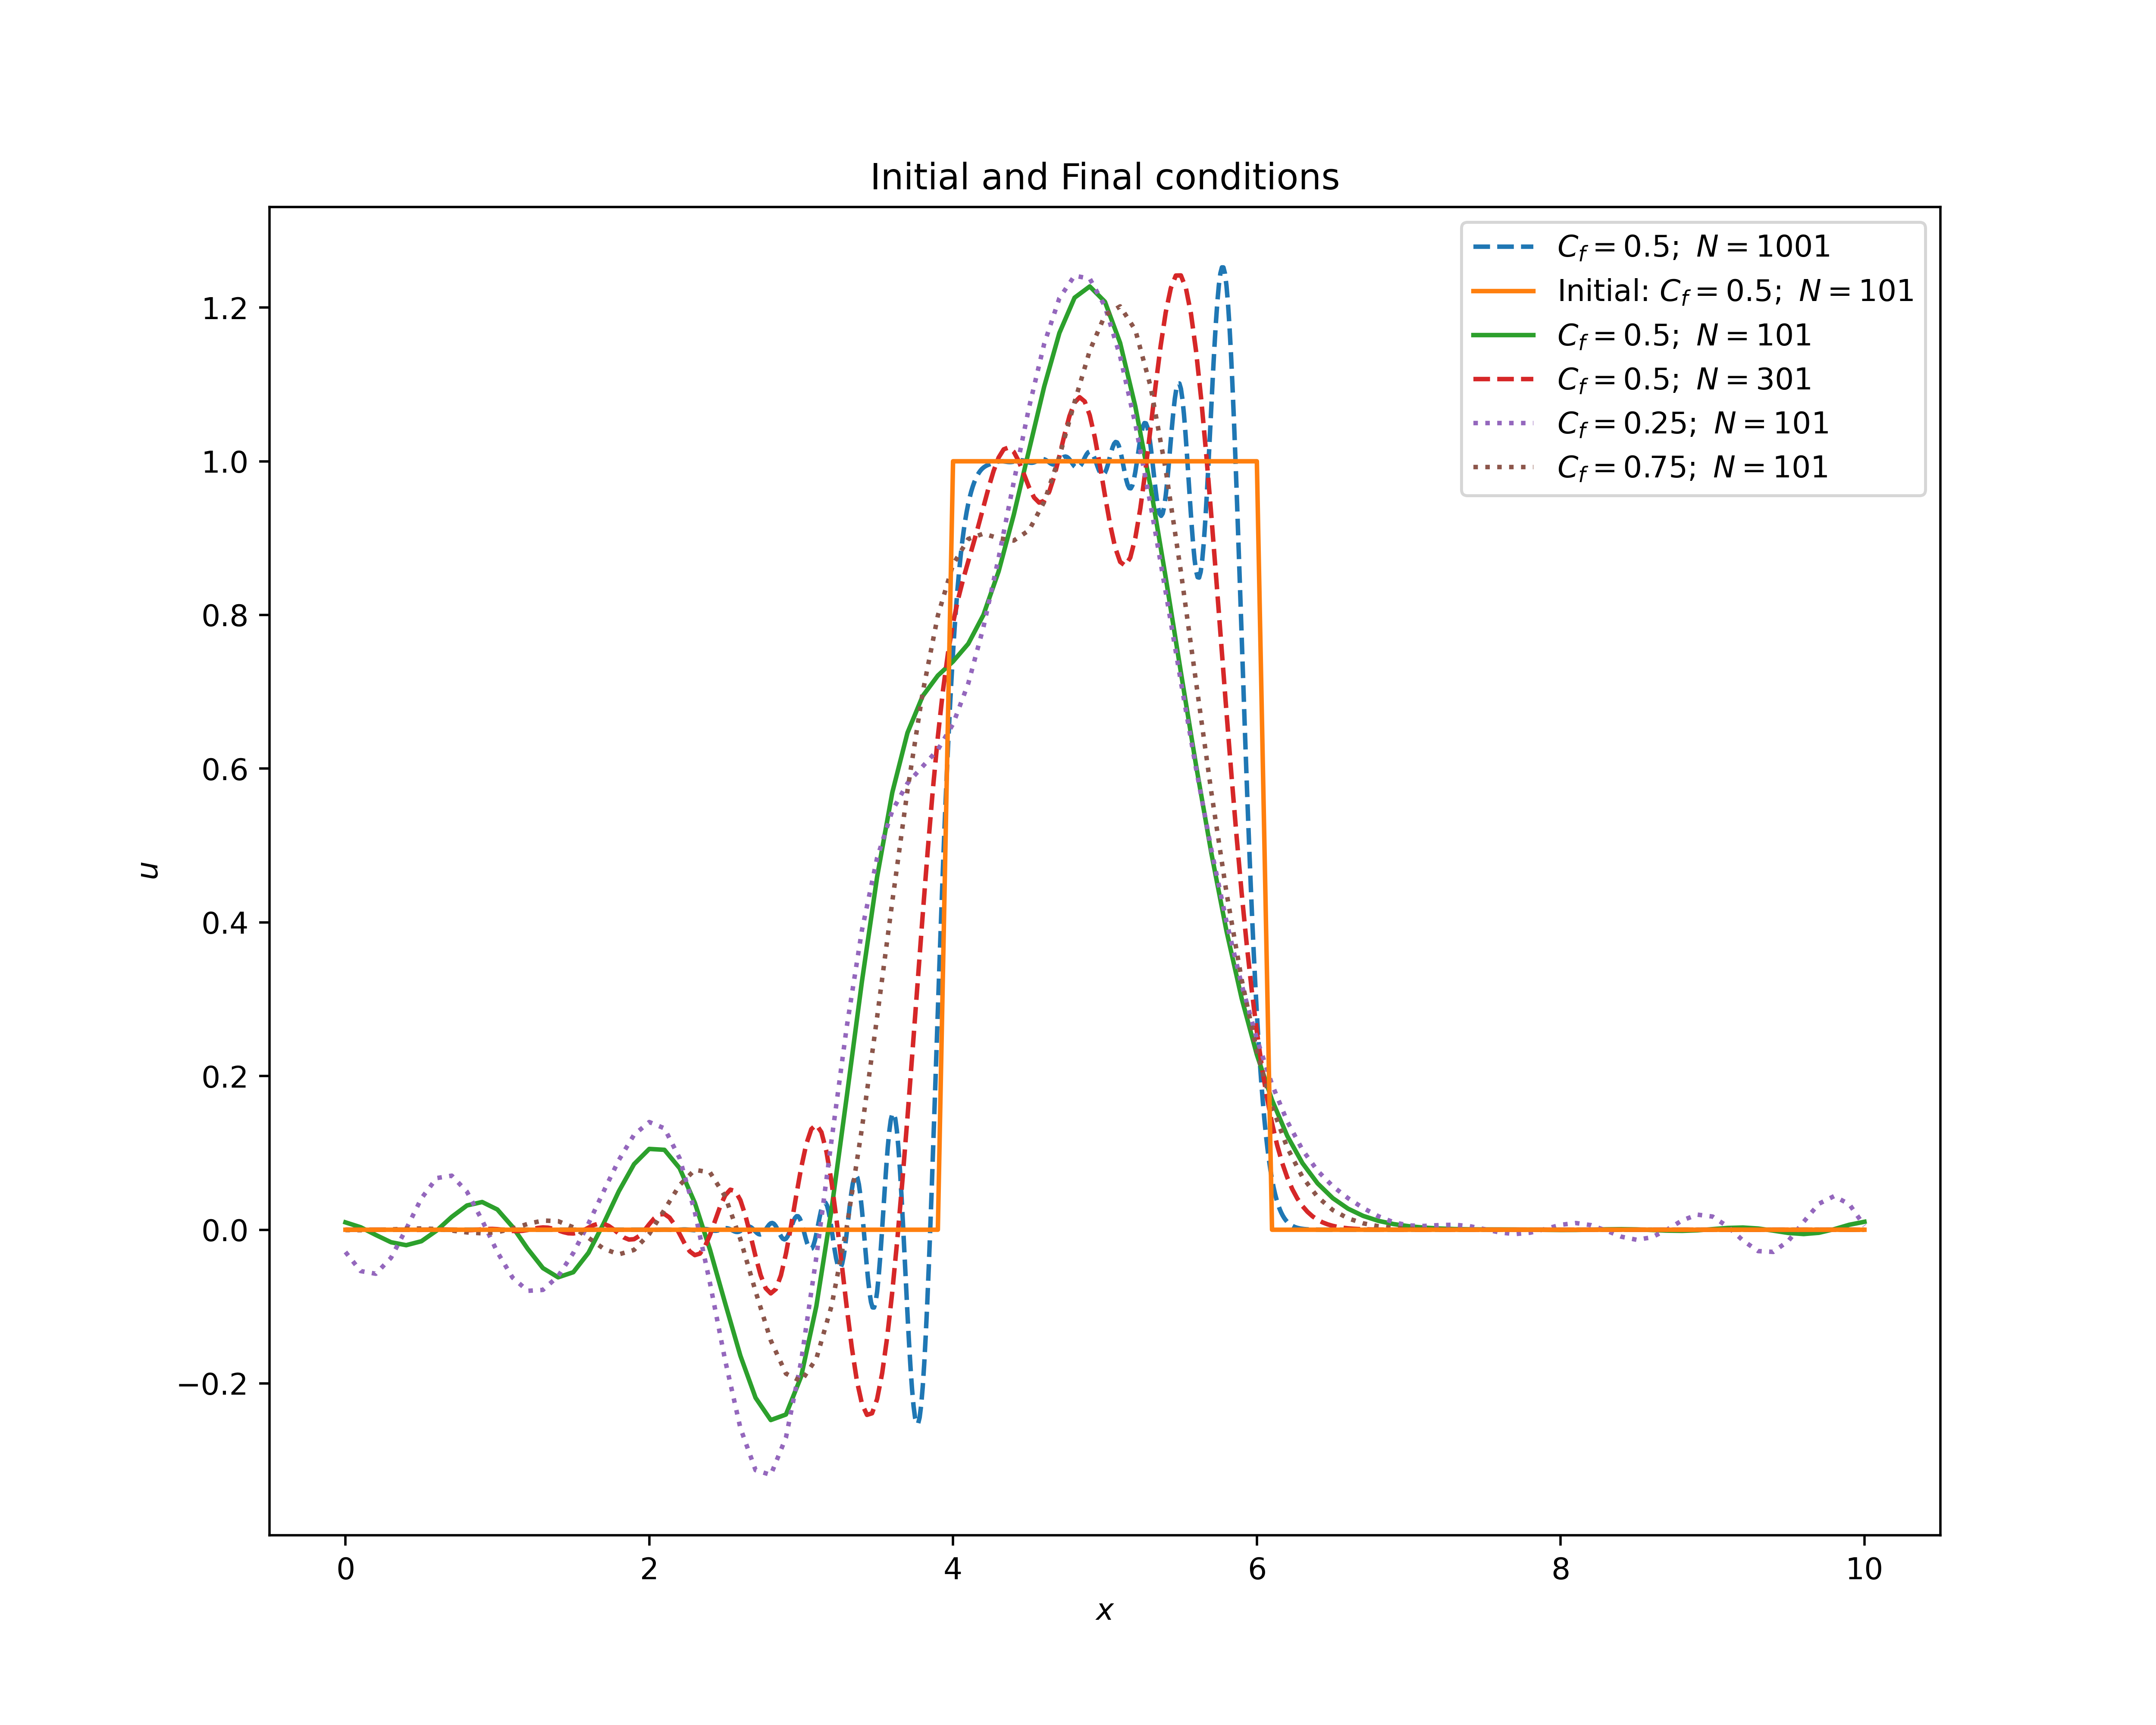
\includegraphics[width=0.9\linewidth]{images/IF_STEP_LAX-W.png}
    \captionof{figure}{Step Function; \acrshort{laxw}; \figifcap.}
    \label{fig:step_laxw_if_tot}
\end{center}

\begin{center}
    \centering
    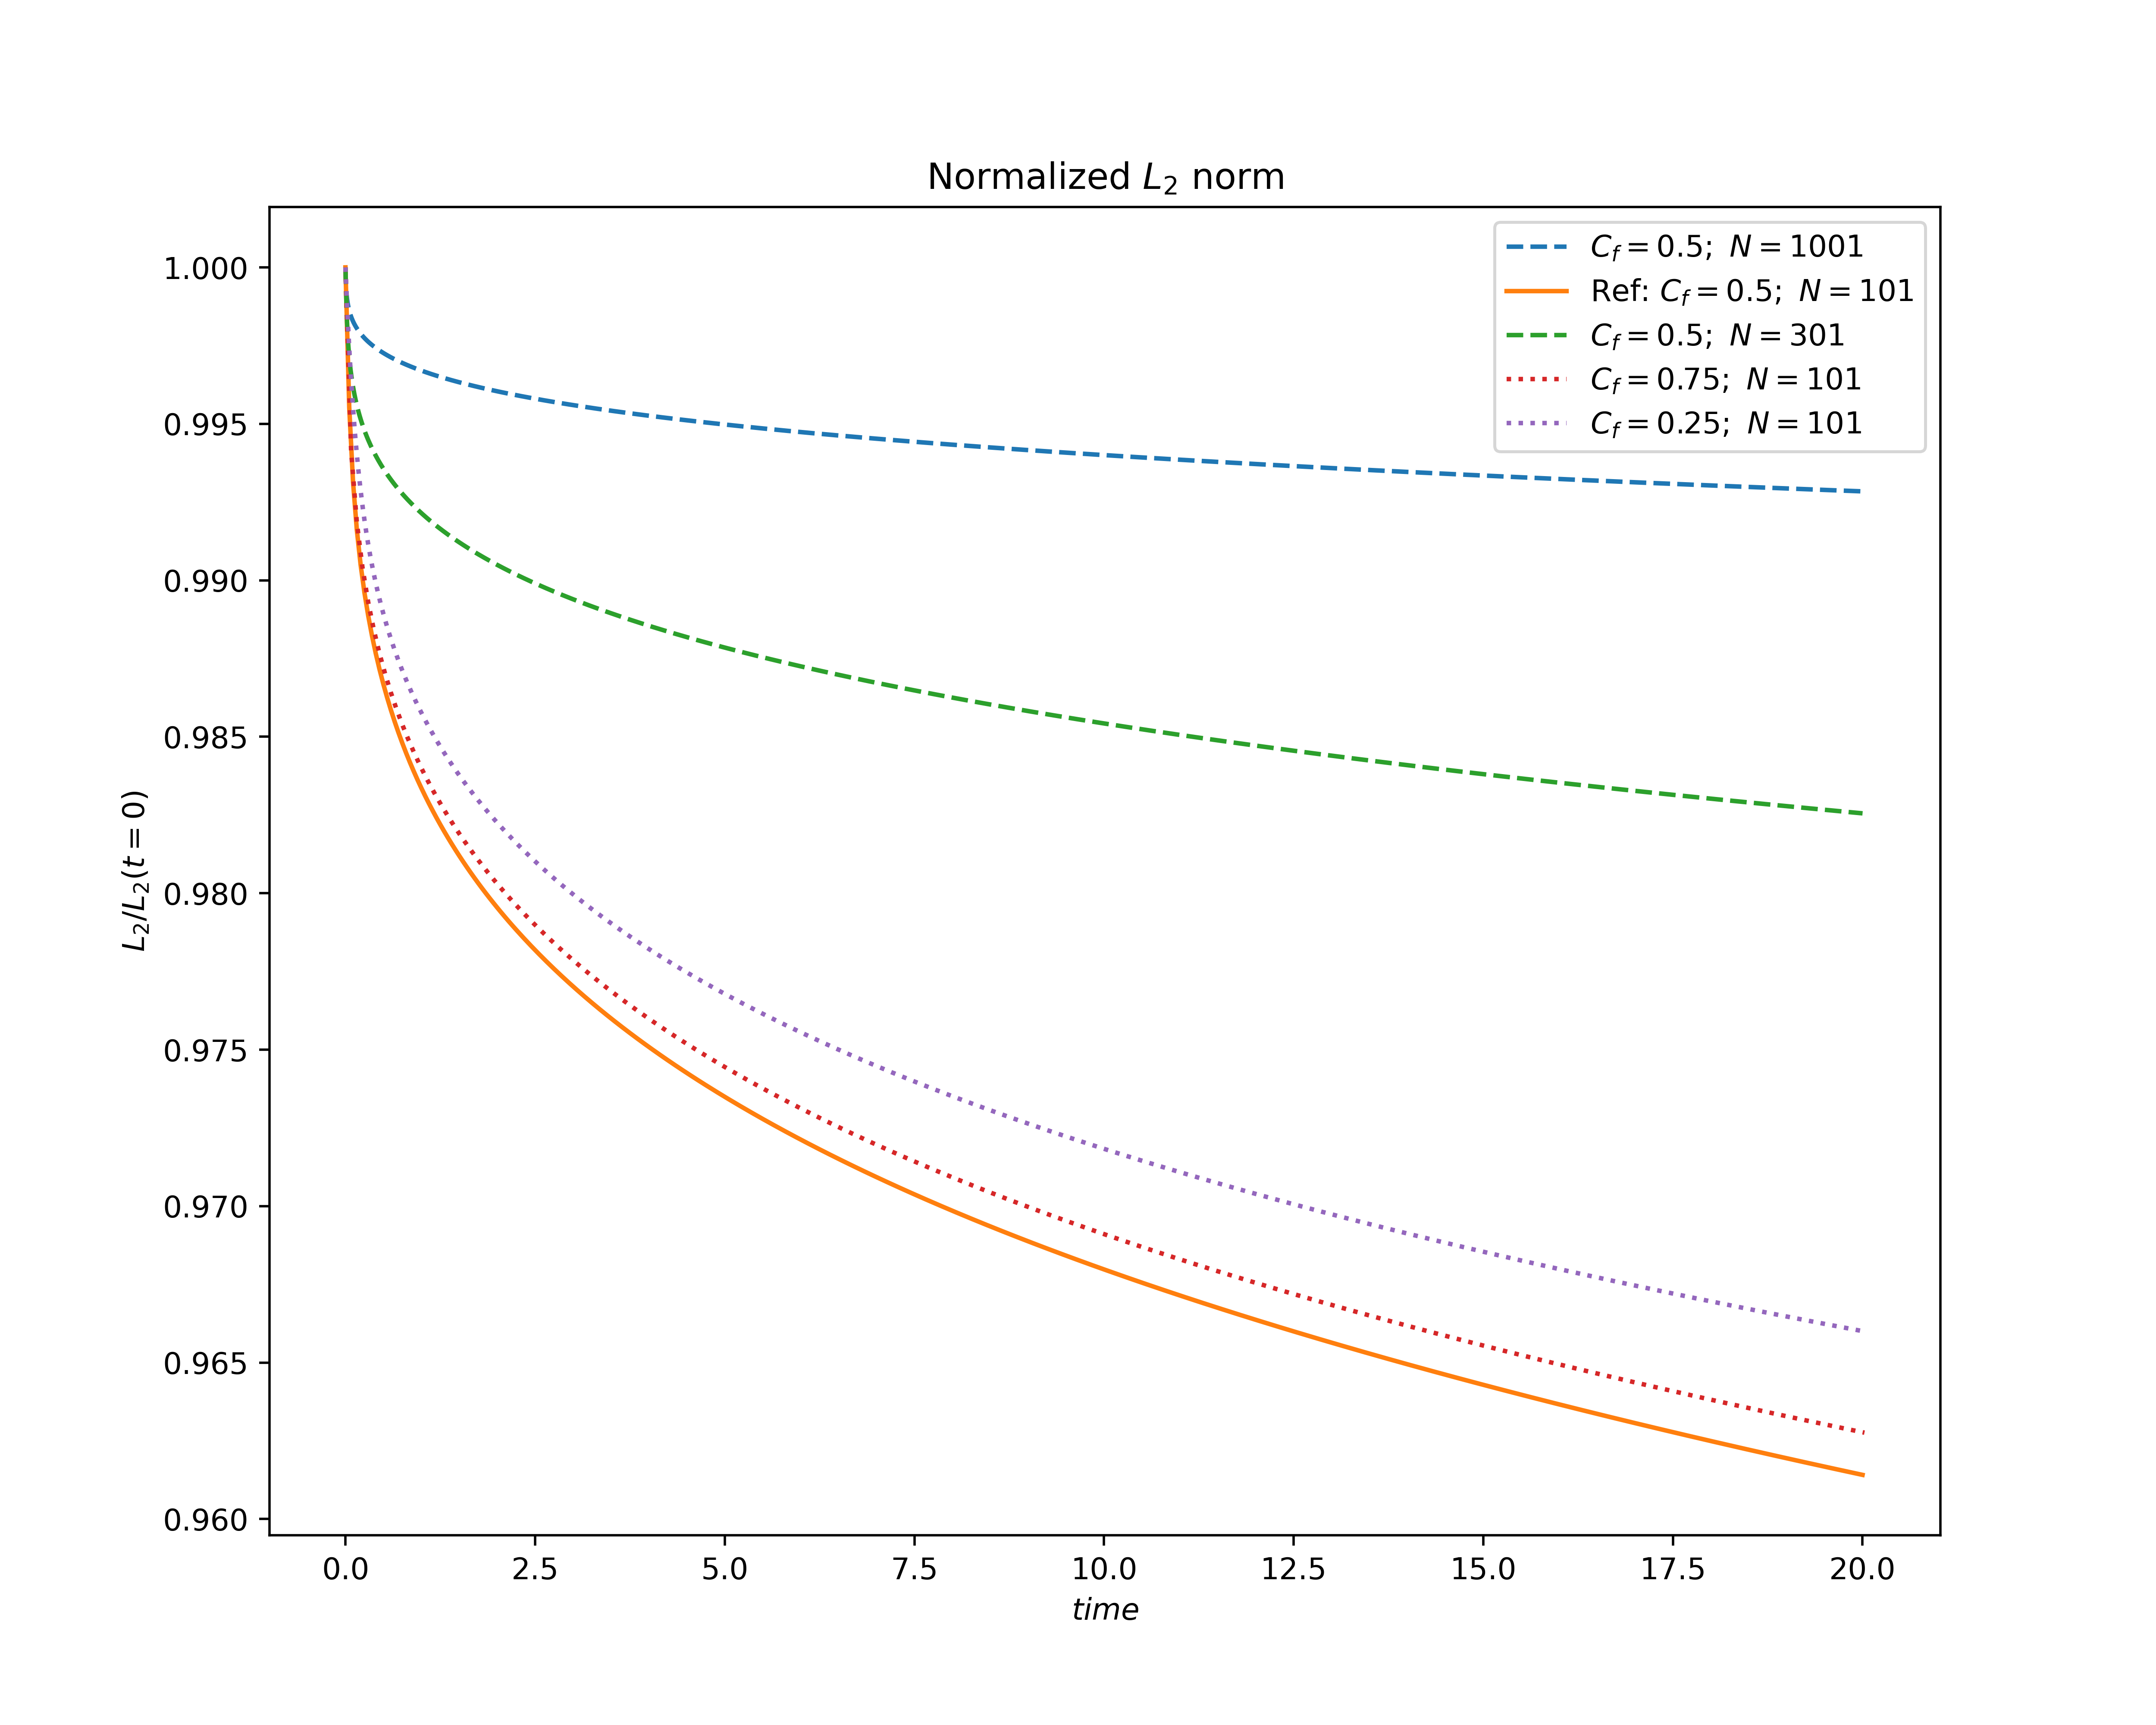
\includegraphics[width=0.9\linewidth]{images/L2_STEP_LAX-W.png}
    \captionof{figure}{Step Function; \acrshort{laxw}; \(L_2\) norm.}
    \label{fig:step_laxw_l2_tot}
\end{center}

\section{\acrfull{beq}}

The \acrlong{beq} is obtained from the \acrlong{aeq} (Equation \ref{eq:adv_eq})
by replacing the (constant) speed \(a\) with \(u\):

\begin{equation} \label{eq:burg_eq_nc}
    \pdv{u}{u} + u \pdv{u}{x} = 0
\end{equation}

\noindent
that is: the speed is not constant anymore, but depends on the amplitude of the
solution. Points at the top have the greatest speed, while point at the bottom
have the smaller (down to speed \(0\) for \(u = 0\)).

The main difference of the \acrshort{beq} from the \acrshort{aeq} is the
formation of new discontinuities. In fact, the \acrshort{aeq} produces just a
translation of the initial solution, meaning that you end up with a discontinuity
at the end just if you had one at the beginning. That is because every point
travels at the same speed. On the other hand, the \acrshort{beq} might produce
a discontinuity even if you started with a smooth solution. The reason is that
since points at different heights have different velocities, the ones that start
behind others but are faster might catch up and form a \textit{shockwave}
(a discontinuity).

Equation \ref{eq:burg_eq_nc} is written in the
\textbf{\acrfull{nfc} Form}. It can be rewritten into Equation
\ref{eq:burg_eq_c}, which is the \textbf{\acrfull{fc} Form}:

\begin{equation} \label{eq:burg_eq_c}
    \pdv{u}{u} + \pdv{f(u)}{x} = 0
\end{equation}

\noindent
where \(f(u) = u^2 / 2\). The difference between the two is relevant because
of the \textbf{Hou - Le Floch Theorem}:

\begin{quote}
    \acrlong{nfc} numerical methods do not converge to the correct
    solution if a shockwave is present.
\end{quote}

\noindent
The expectation is that the solution computed using a \acrshort{fc} or a
\acrshort{nfc} scheme are different. Consider now the
\textbf{Lax-Wendroff Theorem}:

\begin{quote}
    If a consistent numerical method written in a \acrshort{fc} form
    converge to a function \(u(x,\ t)\) for \(\Delta x \to 0\), then
    \(u(x,\ t)\) is a solution of the conservation law.
\end{quote}

\noindent
Therefore if the solution computed with the \acrshort{fc} method converges when
increasing the resolution it has to be the correct one, while the
\acrshort{nfc} version will be different.

For this exercise the initial condition is again a \textbf{Gaussian profile}
set to \(u(t = 0,\ x) = 10 \exp(-(x - x_0)^2)\) with \(x_0 = 5\), to be
solved on a grid with extent \(x \in [0, 10]\) up to \(t = 0.5\).
The Courant factor is set to \(C_f = 0.5\) and initially the number of points
is \(J = 101\). We have checked the behavior of the solutions computed with the
\acrshort{fc} and the \acrshort{nfc} versions of the \textbf{Upwind scheme}
varying the resolution. For simplicity, since we knew in advance that the
solution doesn't grow in amplitude, we set the time step taking into account
the maximum possible velocity:
\(\Delta t = C_f \frac{\Delta x}{\max(u(t = 0,\ x))}\), with
\(\Delta x = 10 / (J - 1)\).

\subsection{Upwind - \acrlong{fc}}

\begin{equation} \label{eq:up-fc}
    u^{n+1}_j = u^n_j - \frac{\Delta t}{2 \Delta x} \qty[(u^n_j)^2 - (u^n_{j-1})^2]
\end{equation}

We will take the \acrshort{fc} scenario to showcase the evolution of the
initial Gaussian profile under the \acrshort{beq} (Figure \ref{fig:up_fc_snap}).
As time advance the points on top of the gaussian travel more than the ones at
the bottom, leading to the formation of a shockwave, like we described above.
Figure \ref{fig:up_fc_if_tot} shows the solutions computed at the final time
using different resolutions. As can be seen, a higher resolution leads to a
steeper and more refined discontinuity. This is expected because the method is
catching the fine details with better precision.

\begin{center}
    \centering
    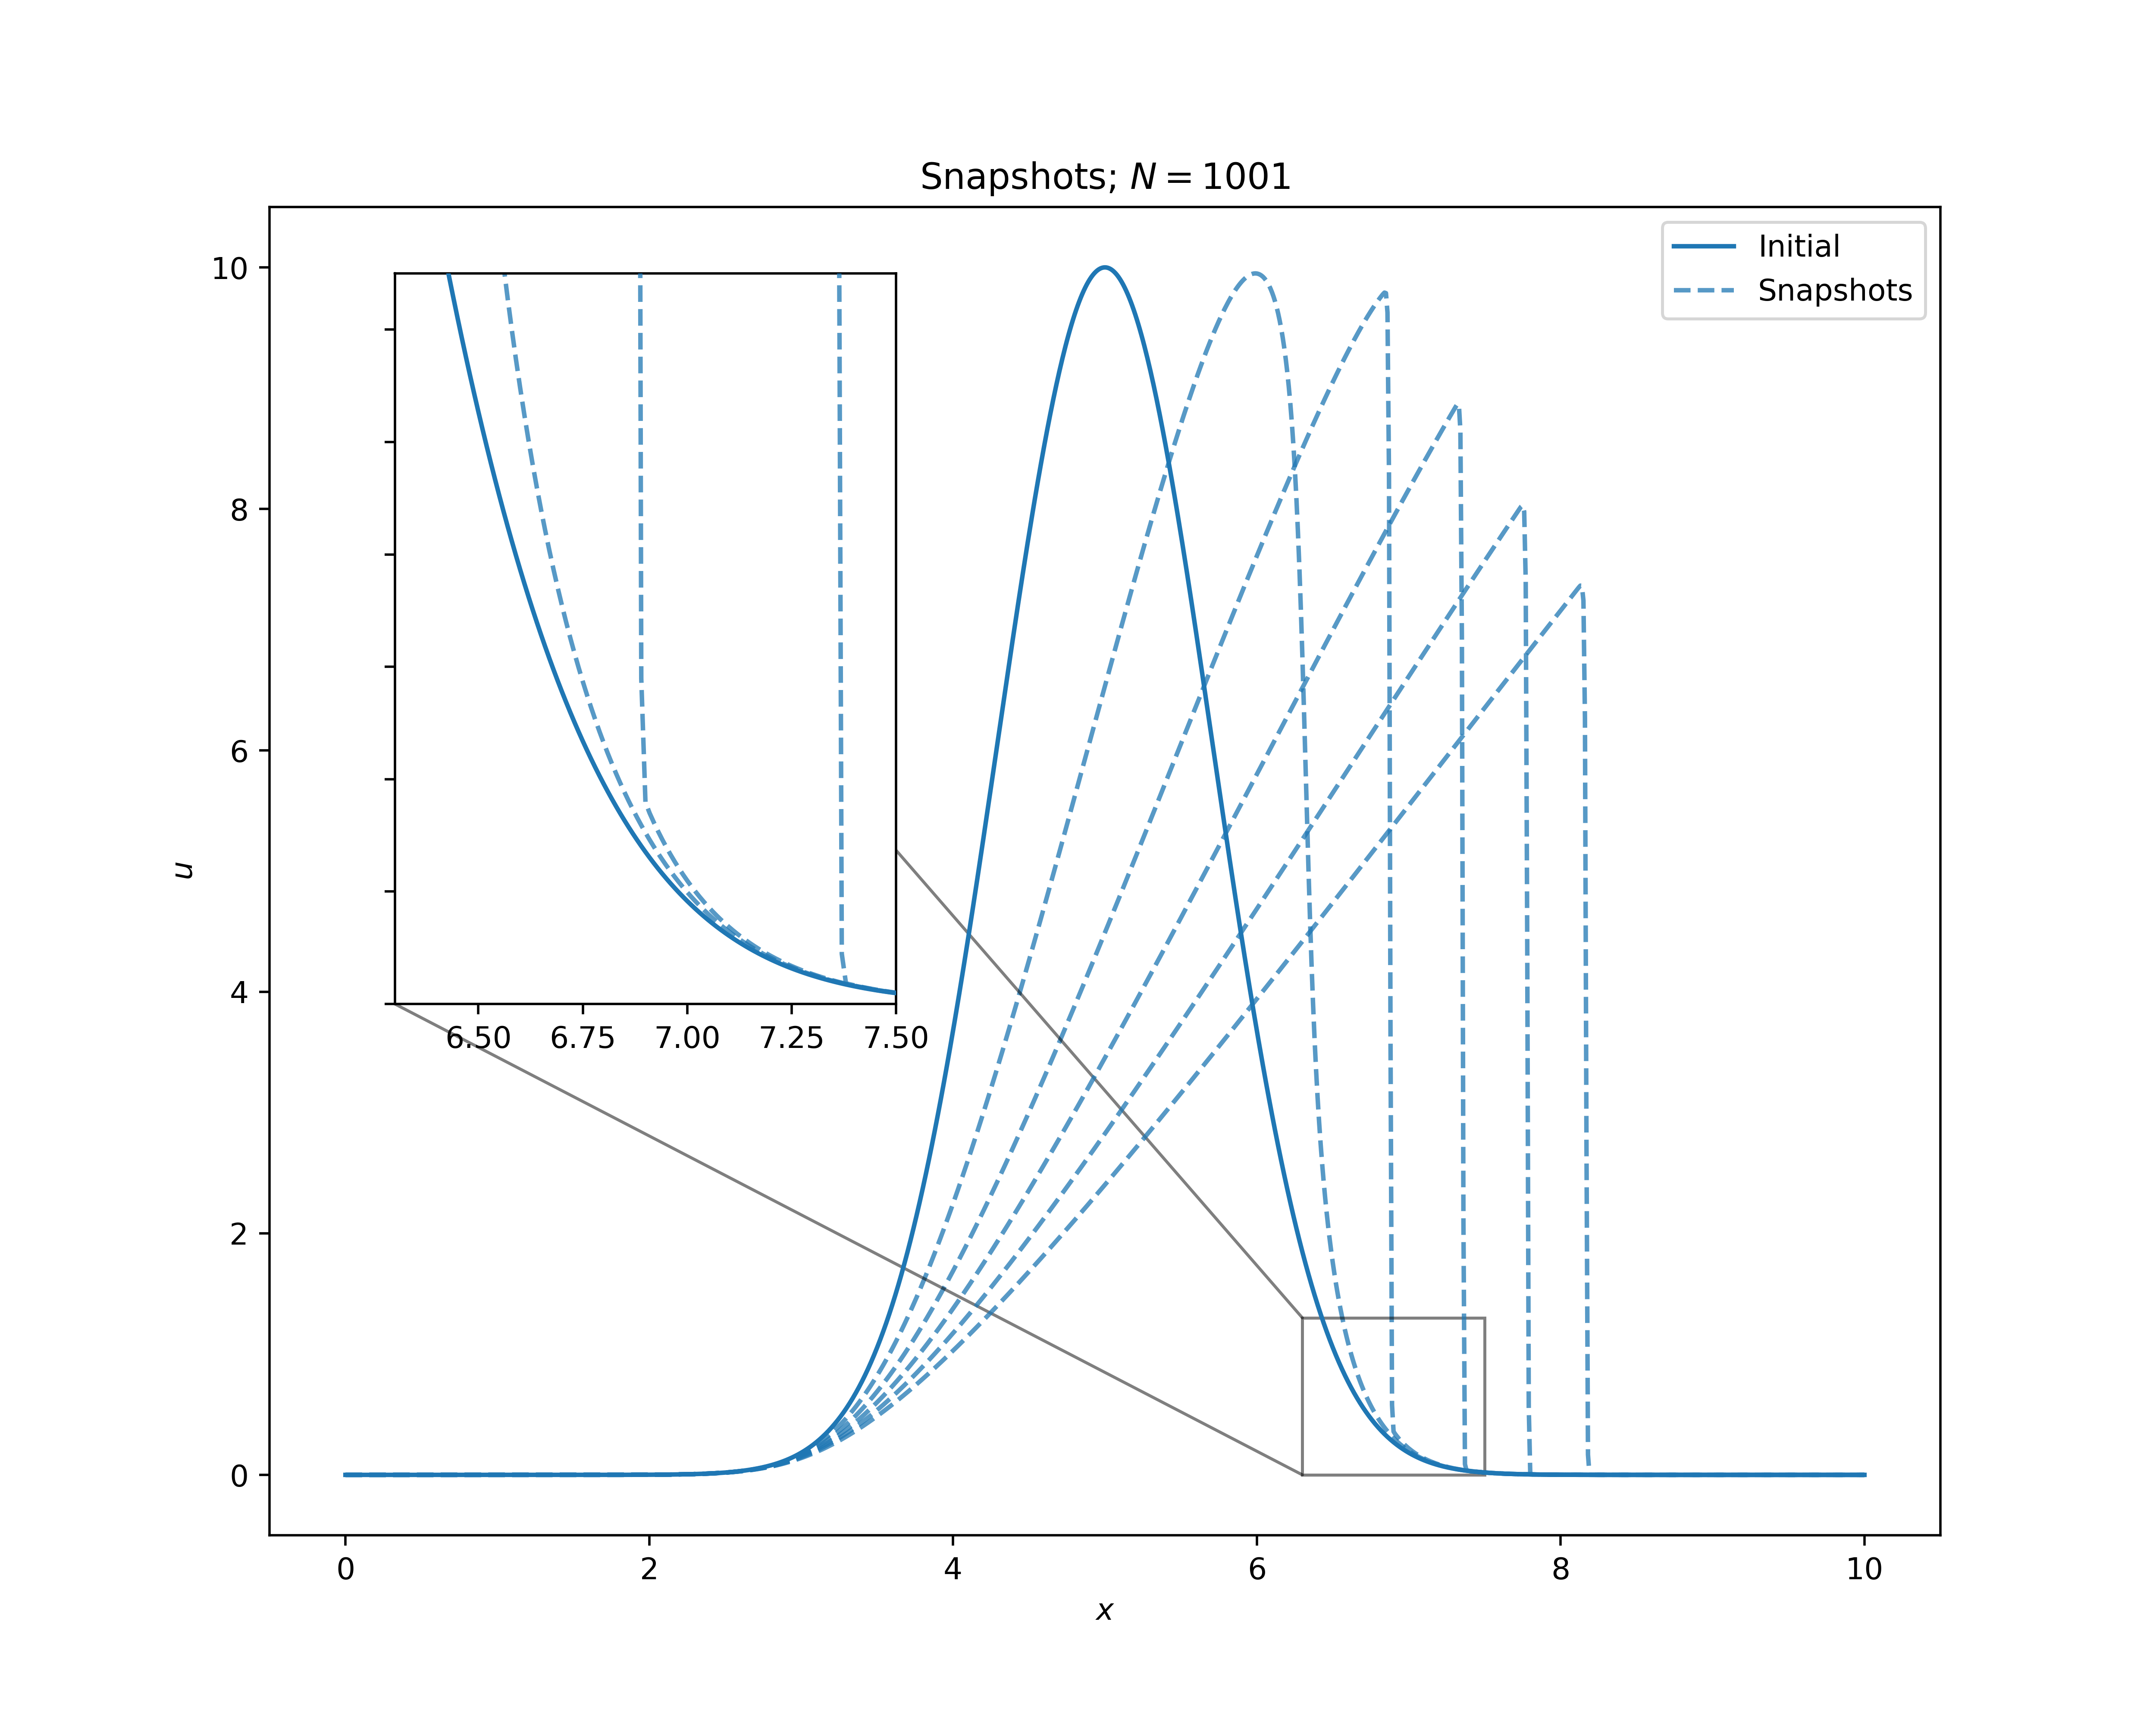
\includegraphics[width=0.9\linewidth]{images/IF_1001_UPWIND-FC.png}
    \captionof{figure}{Upwind - \acrshort{fc}; Snapshots of the solution at different times.}
    \label{fig:up_fc_snap}
\end{center}

\begin{center}
    \centering
    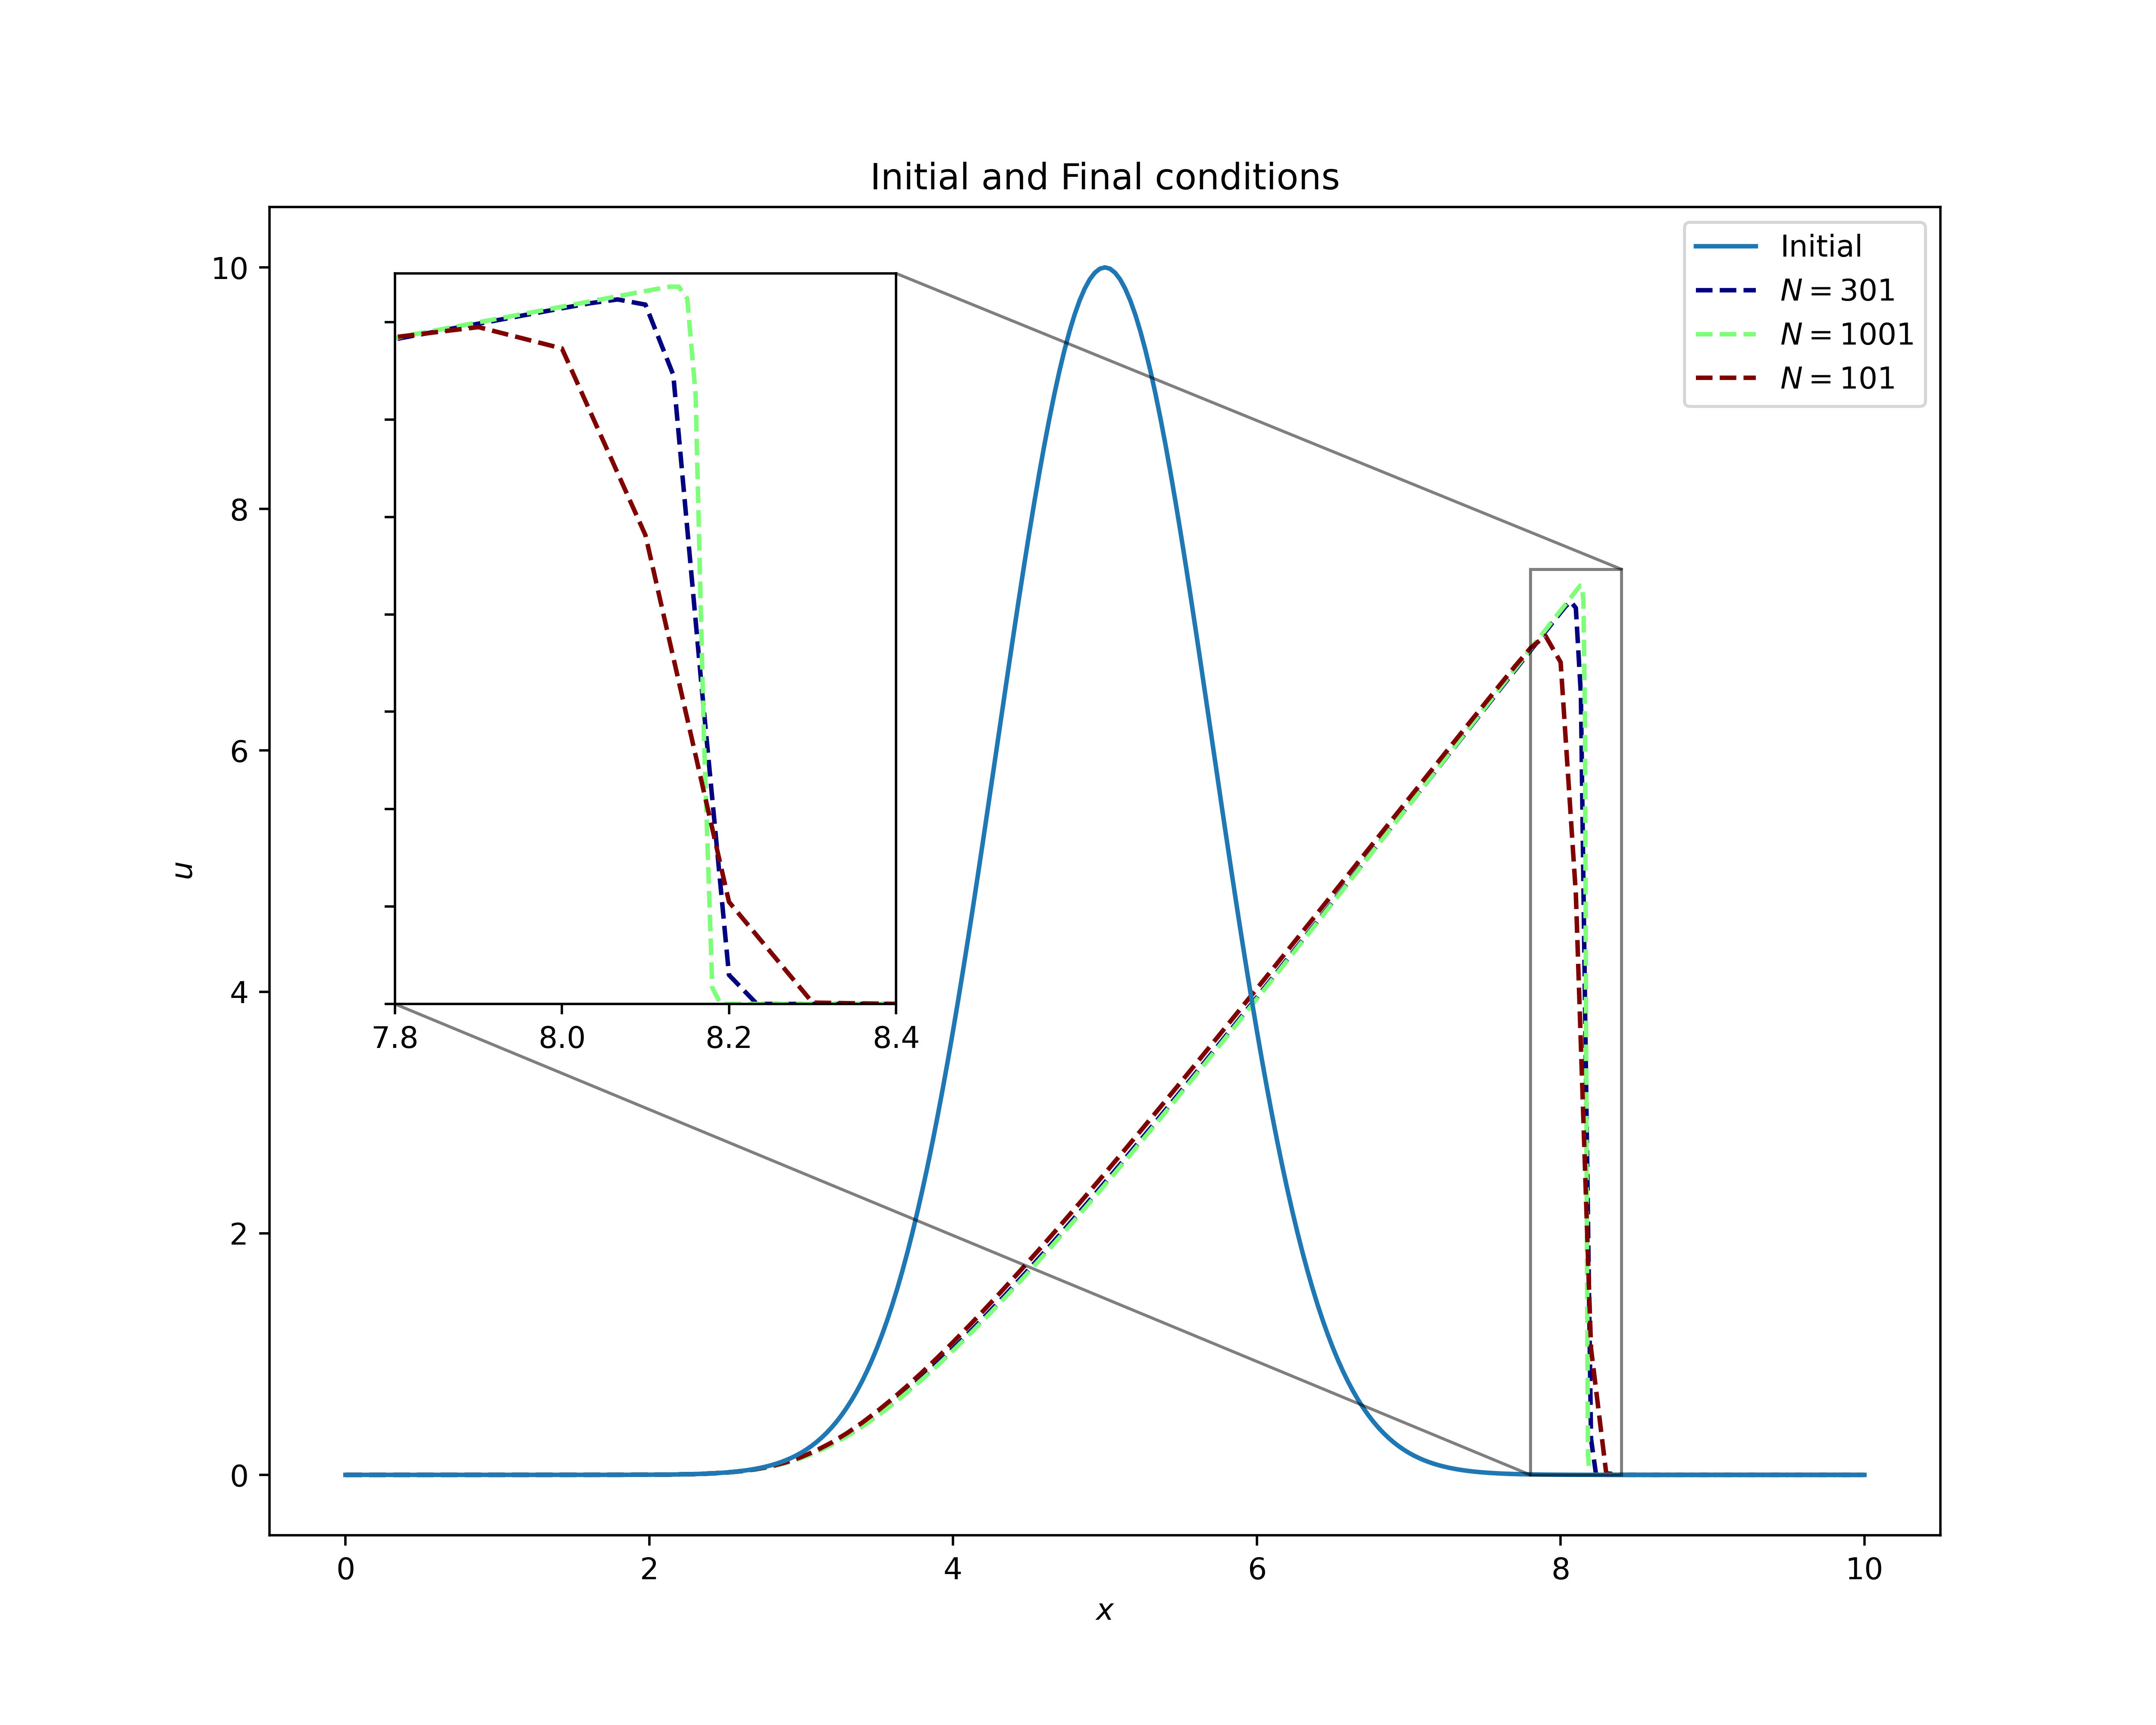
\includegraphics[width=0.9\linewidth]{images/IF_UPWIND-FC.png}
    \captionof{figure}{Upwind - \acrshort{fc}; \figifcap.}
    \label{fig:up_fc_if_tot}
\end{center}

\subsection{Upwind - \acrlong{nfc}}

\begin{equation} \label{eq:up-nfc}
    u^{n+1}_j = u^n_j - \frac{\Delta t}{\Delta x} u^n_j (u^n_j - u^n_{j-1})
\end{equation}

Now we can have a look at the \acrshort{nfc} scenario. The evolution until the
final time is similar to the one in the \acrshort{fc} case, so we will focus
on the differences between the two methods. Figure \ref{fig:up_nfc_if_tot}
shows the obtained initial and final conditions. The situation is analogous to
the previous one, but from Figure \ref{fig:up_comb_if_tot} is clear that the
solutions computed with the two methods don't coincide. As explained before,
this behavior is expected due to the Hou - Le Floch Theorem. Increasing the
resolution wouldn't cause the \acrshort{nfc} solution to shift towards the
\acrshort{fc} one, which instead is correct by virtue of the
Lax-Wendroff Theorem.

\begin{center}
    \centering
    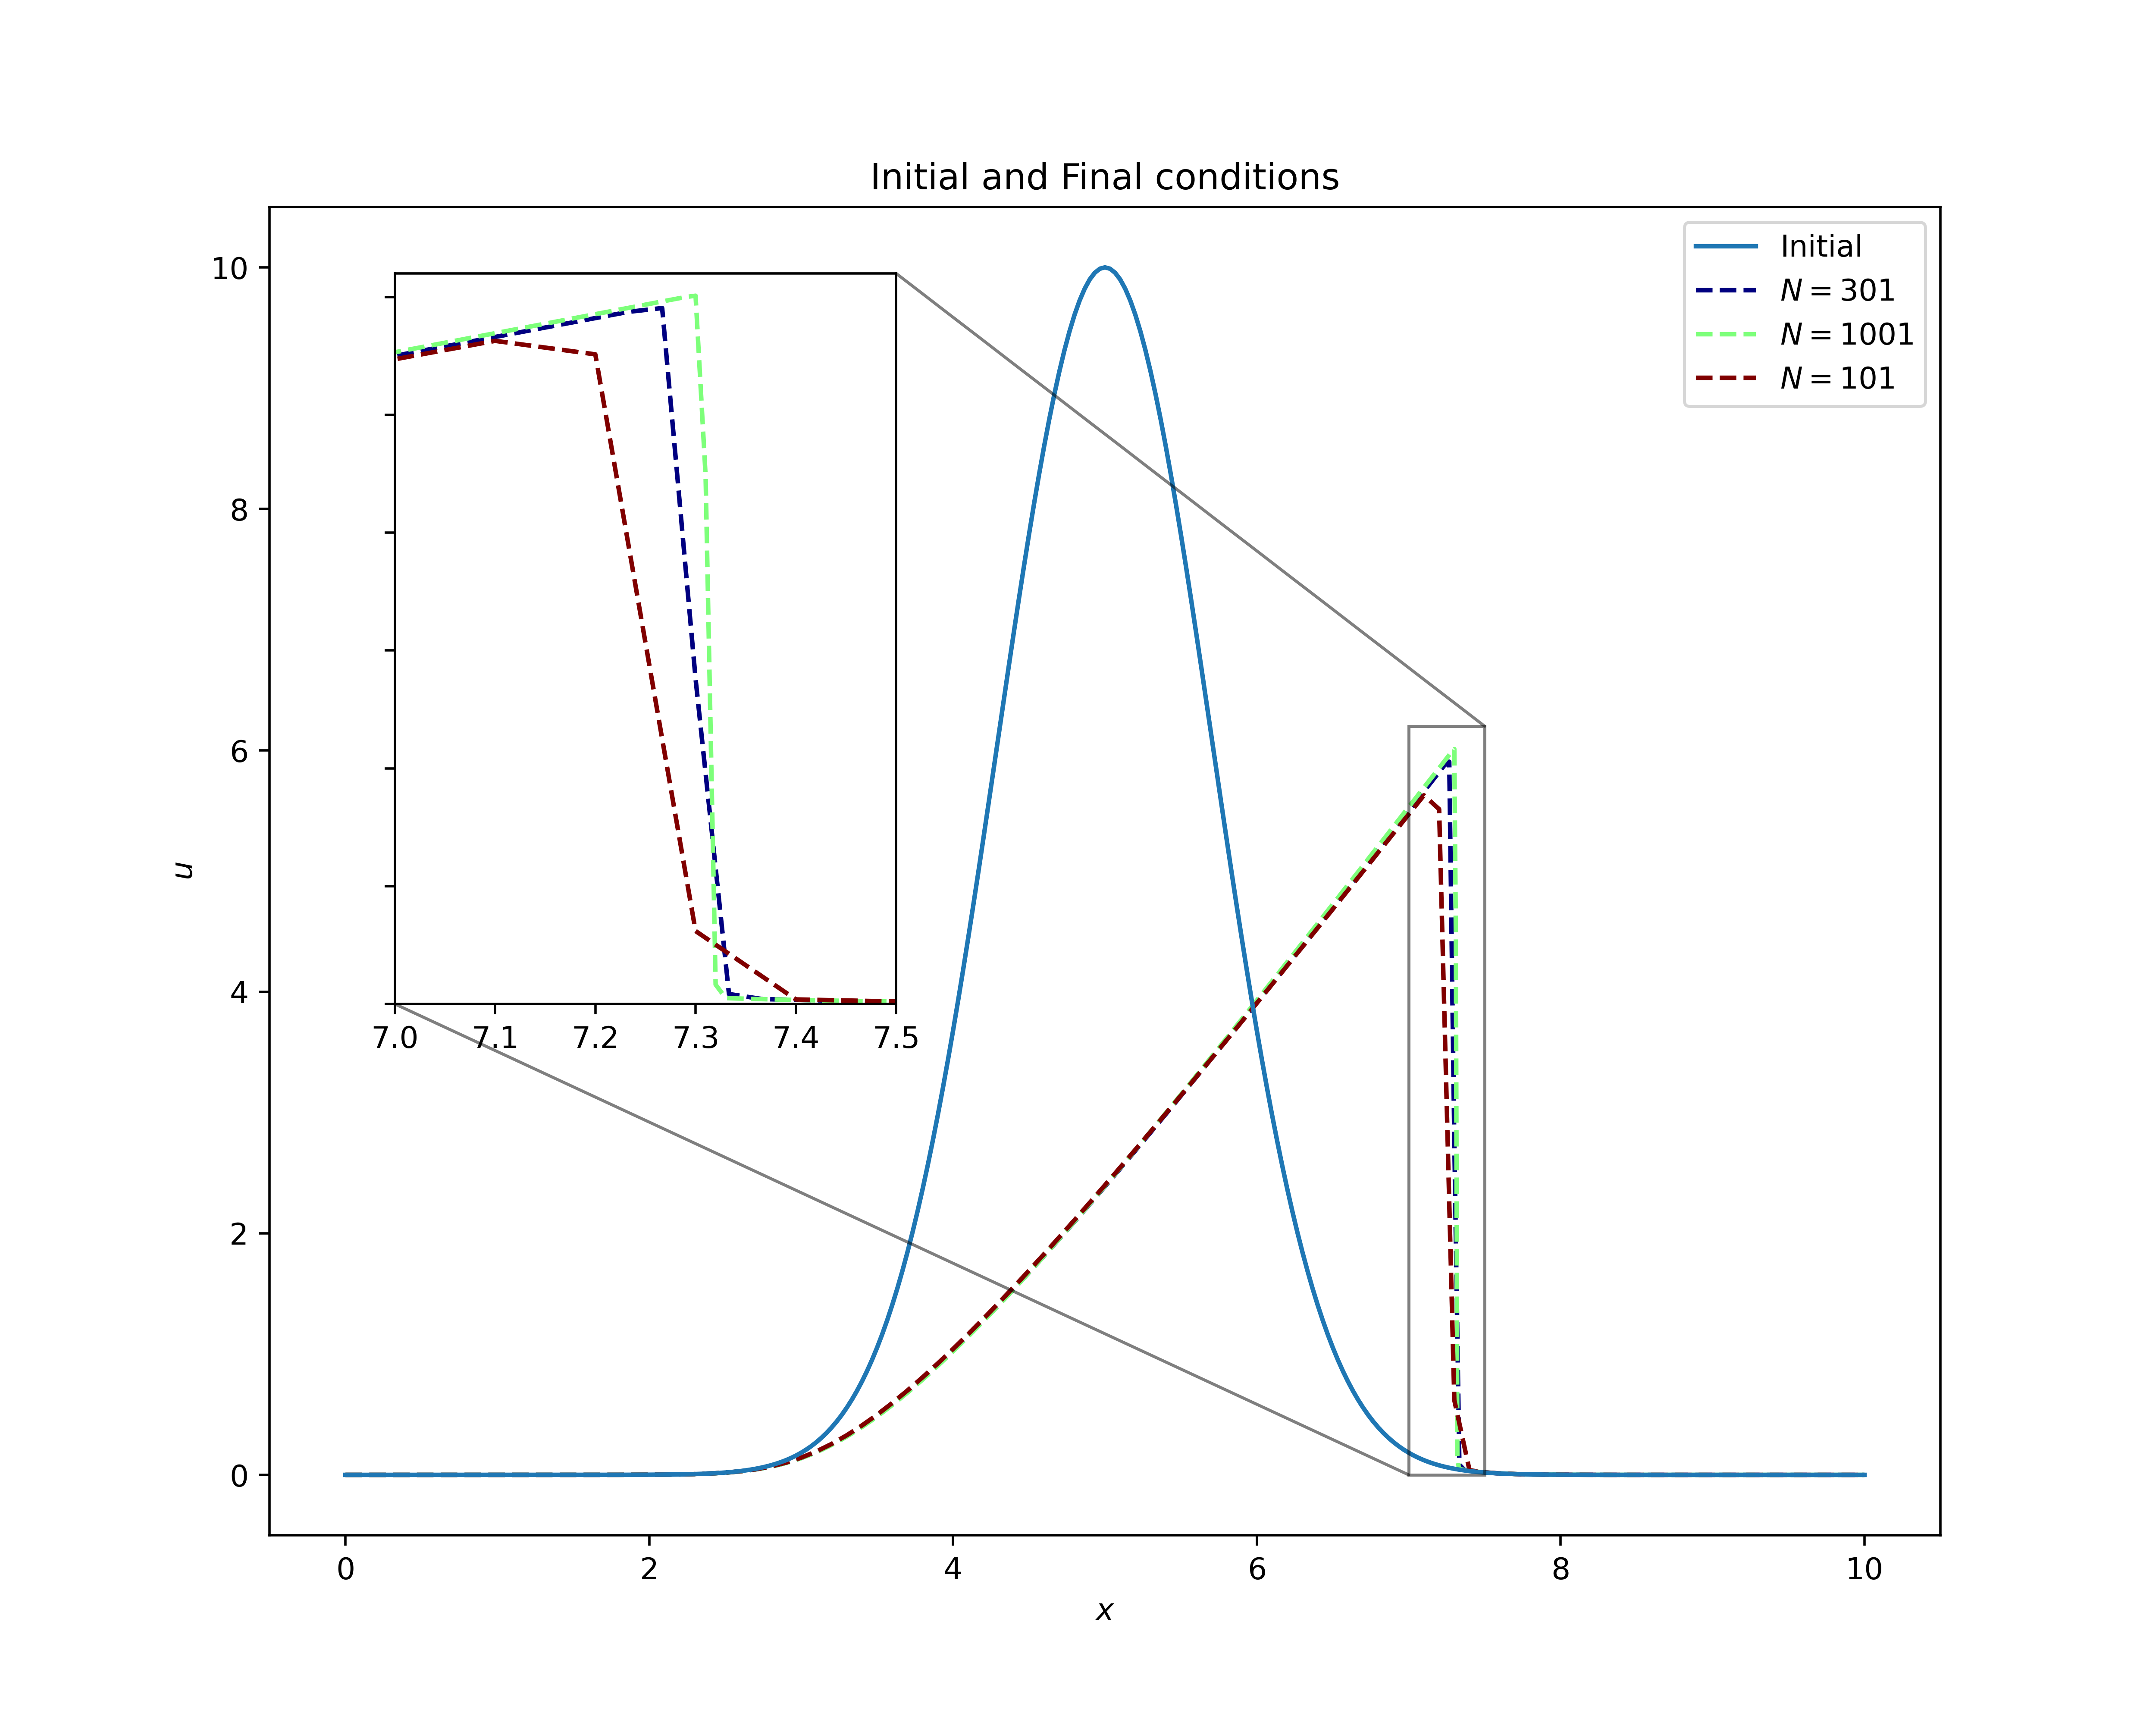
\includegraphics[width=0.9\linewidth]{images/IF_UPWIND-NFC.png}
    \captionof{figure}{Upwind - \acrshort{nfc}; \figifcap.}
    \label{fig:up_nfc_if_tot}
\end{center}

\begin{center}
    \centering
    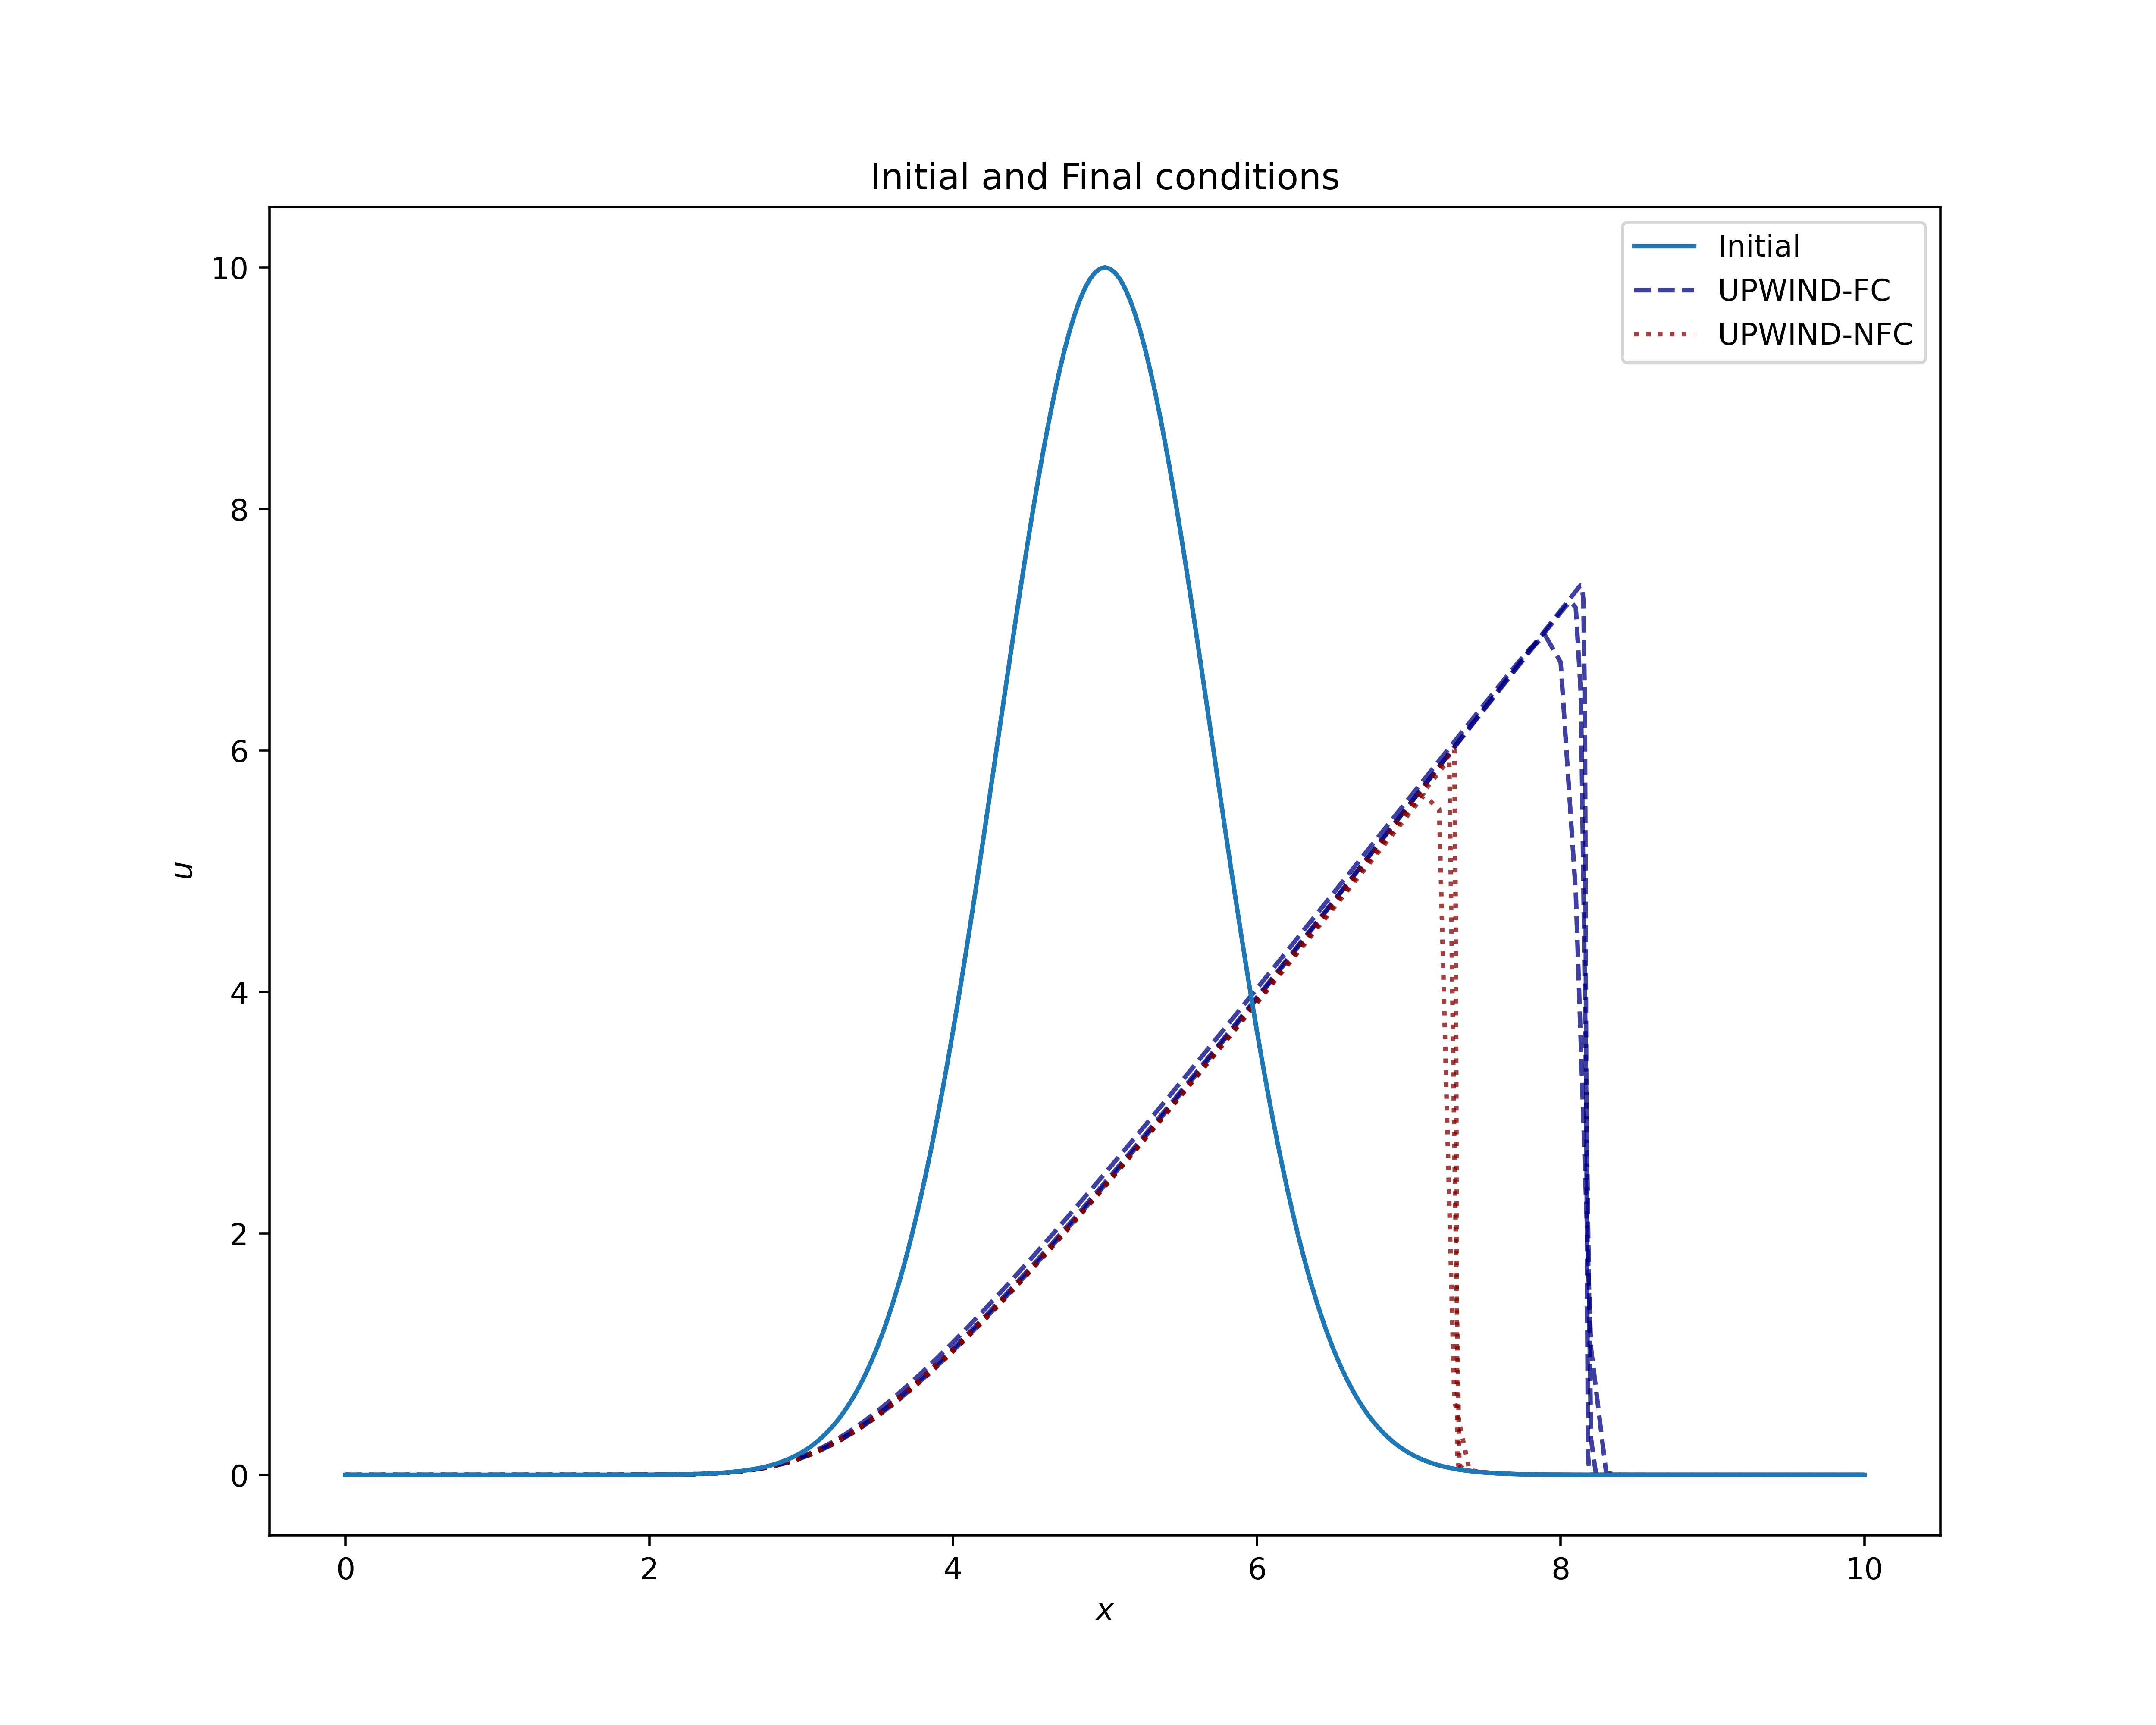
\includegraphics[width=0.9\linewidth]{images/IF_UPWIND_COMBINED.png}
    \captionof{figure}{\figifcap; \acrshort{fc} and \acrshort{nfc} Upwind combined.}
    \label{fig:up_comb_if_tot}
\end{center}

\end{document}
